% /*
%  * ----------------------------------------------------------------------------
%  * "THE BEER-WARE LICENSE" (Revision 42):
%  * Julian Klaiber and Severin Dellsperger wrote this file. As long as you retain this notice you
%  * can do whatever you want with this stuff. If we meet some day, and you think
%  * this stuff is worth it, you can buy us a beer in return.
%  * ----------------------------------------------------------------------------
%  */

% Template Informationen
\documentclass[
a4paper,
oneside,
10pt,
fleqn,
headsepline,
toc=listofnumbered, 
bibliography=totocnumbered]{scrartcl}

% deutsche Trennmuster etc.
\usepackage[T1]{fontenc}
\usepackage[utf8]{inputenc}
\usepackage[english, ngerman]{babel} % \selectlanguage{english} if  needed
\usepackage{lmodern} % use modern latin fonts

% Custom commands
\newcommand{\GITHUB}{https://github.com/jklaiber/HSR}
\newcommand{\LICENSEURL}{https://en.wikipedia.org/wiki/Beerware}
\newcommand{\LICENSE}{
"THE BEER-WARE LICENSE" (Revision 42):
Julian Klaiber and Severin Dellsperger wrote this file. As long as you retain this notice you
can do whatever you want with this stuff. If we meet some day, and you think
this stuff is worth it, you can buy us a beer in return.
}

% Jede Überschrift 1 auf neuer Seite
\let\stdsection\section
\renewcommand\section{\clearpage\stdsection}

% Multiple Authors
\usepackage{authblk}

% Include external pdf
\usepackage{pdfpages}

% Layout / Seitenränder
\usepackage{geometry}

% Inhaltsverzeichnis
\usepackage{makeidx} 
\makeindex

\usepackage{url}
\usepackage[pdfborder={0 0 0}]{hyperref}
\usepackage[all]{hypcap}
\usepackage{hyperxmp} % for license metadata

% Glossar und Abkürzungsverzeichnis
\usepackage[acronym,toc,nopostdot]{glossaries}
\setglossarystyle{altlist}
\usepackage{xparse}
\DeclareDocumentCommand{\newdualentry}{ O{} O{} m m m m } {
	\newglossaryentry{gls-#3}{
		name={#4 : #5},
		text={#5\glsadd{#3}},
		description={#6},
		#1
	}
	\makeglossaries
	\newacronym[see={[Siehe:]{gls-#3}},#2]{#3}{#4}{#5\glsadd{gls-#3}}
}
\makeglossaries

% Mathematik
\usepackage{amsmath}
\usepackage{amssymb}
\usepackage{amsfonts}
\usepackage{enumitem}

% Images
\usepackage{graphicx}
\graphicspath{{images/}} % default paths

% Boxes
\usepackage{fancybox}

%Tables
\usepackage{tabu}
\usepackage{booktabs} % toprule, midrule, bottomrule
\usepackage{array} % for matrix tables
\usepackage{multicol} %multicol

% Header and footer
\usepackage{scrlayer-scrpage}
\setkomafont{pagehead}{\normalfont}
\setkomafont{pagefoot}{\normalfont}
\automark*{section}
\clearpairofpagestyles
\ihead{\headmark}
\ohead{\AUTHOR}
\cfoot{\pagemark}

% Pseudocode
\usepackage{algorithmic}
\usepackage[linesnumbered,ruled]{algorithm2e}

% Code Listings
\usepackage{listings}
\usepackage{color}
\usepackage{beramono}

\definecolor{bluekeywords}{rgb}{0,0,1}
\definecolor{greencomments}{rgb}{0,0.5,0}
\definecolor{redstrings}{rgb}{0.64,0.08,0.08}
\definecolor{xmlcomments}{rgb}{0.5,0.5,0.5}
\definecolor{types}{rgb}{0.17,0.57,0.68}

\lstdefinestyle{visual-studio-style}{
	language=[Sharp]C,
	columns=flexible,
	showstringspaces=false,
	basicstyle=\footnotesize\ttfamily, 
	commentstyle=\color{greencomments},
	morekeywords={partial, var, value, get, set},
	keywordstyle=\bfseries\color{bluekeywords},
	stringstyle=\color{redstrings},
	breaklines=true,
	breakatwhitespace=true,
	tabsize=4,
	numbers=left,
	numberstyle=\tiny\color{black},
	frame=lines,
	showspaces=false,
	showtabs=false,
	escapeinside={£}{£},
}

\definecolor{DarkPurple}{rgb}{0.4, 0.1, 0.4}
\definecolor{DarkCyan}{rgb}{0.0, 0.5, 0.4}
\definecolor{LightLime}{rgb}{0.3, 0.5, 0.4}
\definecolor{Blue}{rgb}{0.0, 0.0, 1.0}

\lstdefinestyle{cevelop-style}{
	language=C++,  
	columns=flexible,
	showstringspaces=false,     
	basicstyle=\footnotesize\ttfamily, 
	keywordstyle=\bfseries\color{DarkPurple},
	commentstyle=\color{LightLime},
	stringstyle=\color{Blue}, 
	escapeinside={£}{£}, % latex scope within code      
	breaklines=true,
	breakatwhitespace=true,
	showspaces=false,
	showtabs=false,
	tabsize=4,
	morekeywords={include,ifndef,define},
	numbers=left,
	numberstyle=\tiny\color{black},
	frame=lines,
}

\lstdefinestyle{eclipse-style}{
	language=Java,  
	columns=flexible,
	showstringspaces=false,     
	basicstyle=\footnotesize\ttfamily, 
	keywordstyle=\bfseries\color{DarkPurple},
	commentstyle=\color{LightLime},
	stringstyle=\color{Blue}, 
	escapeinside={£}{£}, % latex scope within code      
	breaklines=true,
	breakatwhitespace=true,
	showspaces=false,
	showtabs=false,
	tabsize=4,
	morekeywords={length},
	numbers=left,
	numberstyle=\tiny\color{black},
	frame=lines,
}
\lstset{style=eclipse-style}



% Theorems \begin{mytheo}{title}{label}
\usepackage{tcolorbox}
\tcbuselibrary{theorems}
\newtcbtheorem[number within=section]{definiton}{Definition}%
{fonttitle=\bfseries}{def}
\newtcbtheorem[number within=section]{remember}{Merke}%
{fonttitle=\bfseries}{rem}
\newtcbtheorem[number within=section]{hint}{Hinweis}%
{fonttitle=\bfseries}{hnt}

% Colors
\definecolor{strings}{HTML}{448c25}
\definecolor{comments}{HTML}{aaaaaa}
\definecolor{keywords}{HTML}{aa3d8c}
\definecolor{background}{HTML}{f4f4f4}
\definecolor{numbers}{HTML}{a884e0}

% Default style
\lstdefinestyle{default}{
    backgroundcolor=\color{background},
    basicstyle=\ttfamily\small,
    breakatwhitespace=true,
    breaklines=true,
    commentstyle=\color{comments},
    deletekeywords={},
    escapeinside={}{},
    extendedchars=true,
    frame=lines,
    keepspaces=true,
    keywordstyle=\color{keywords},
    morekeywords={},
    numbers=left,
    numberstyle=\ttfamily\color{numbers},
    rulecolor=\color{numbers},
    showspaces=false,
    showstringspaces=false,
    showtabs=false,
    stepnumber=1,
    stringstyle=\color{strings},
    tabsize=2,
}
\lstset{
    style=default,
    columns=fullflexible
}

% Language cisco-config
\lstdefinelanguage{cisco-config}{
    morekeywords={no,ip,ipv6,int,interface},
    morecomment=[l][\color{comments}]{!},
    numbers=none
}

% Language cisco-teminal
\lstdefinelanguage{cisco-terminal}{
    morecomment=[l][\color{strings}]{\#},
    morecomment=[l][\color{strings}]{>},
    numbers=none
}

\lstdefinelanguage{bash}{
    numbers=none
}

\makeatletter
\@addtoreset{section}{part}
\makeatother

% Boxes
\tcbuselibrary{most}

\usepackage{fontawesome}

% \cmd{...}
\newcommand{\cmd}[1]{\texttt{#1}}

% Info Box
\definecolor{infobar}{HTML}{02cefc}
\definecolor{infobackground}{HTML}{baf0fc}
\newcommand{\info}[2]{
    \begin{tcolorbox}[
        arc = 0mm,
        boxrule = 0pt,
        breakable,
        before skip=11pt,
        before skip=11pt,
        title = \faInfo~#1,
        fonttitle = \sffamily\bfseries,
        coltitle = white,
        colbacktitle = infobar,
        colback = infobackground,
        toptitle=2mm,
        bottomtitle=2mm,
        top=4mm,
        bottom=4mm
    ]
    #2
    \end{tcolorbox}
}

% Warning Box
\definecolor{warnbar}{HTML}{f90053}
\definecolor{warnbackground}{HTML}{fcc4d7}
\newcommand{\warn}[2]{
    \begin{tcolorbox}[
        arc = 0mm,
        boxrule = 0pt,
        breakable,
        before skip=11pt,
        before skip=11pt,
        title = \faWarning~#1,
        fonttitle = \sffamily\bfseries,
        coltitle = white,
        colbacktitle = warnbar,
        colback = warnbackground,
        toptitle=2mm,
        bottomtitle=2mm,
        top=4mm,
        bottom=4mm
    ]
    #2
    \end{tcolorbox}
}

% Login Information Box
\definecolor{loginbar}{HTML}{FA8A05}
\definecolor{loginbackground}{HTML}{F3D4AF}
\newcommand{\login}[2]{
    \begin{tcolorbox}[
        arc = 0mm,
        boxrule = 0pt,
        breakable,
        before skip=11pt,
        before skip=11pt,
        title = \faKey~#1,
        fonttitle = \sffamily\bfseries,
        coltitle = white,
        colbacktitle = loginbar,
        colback = loginbackground,
        toptitle=2mm,
        bottomtitle=2mm,
        top=4mm,
        bottom=4mm
    ]
    #2
    \end{tcolorbox}
}

\definecolor{settingborder}{HTML}{0066CC}
\definecolor{settingcontent}{HTML}{E5F2FA}
\newcommand{\setting}[1]{
    \begin{tcolorbox}[
        colback = settingcontent,
        colframe = settingborder
    ]
    You can find the settings under: \\
    \textbf{\clicks{~#1}}
    \end{tcolorbox}
}

\definecolor{configurationborder}{HTML}{005700}
\definecolor{configurationcontent}{HTML}{e6ffcc}
\newcommand{\configuration}[2]{
    \begin{tcolorbox}[
        colback = configurationcontent,
        colframe = configurationborder
    ]
    \textbf{Configuration:}\\
    To reach an output like below you only have to add/change the following parameters 
    ~#1
    You can find the settings under: \\
    \textbf{\clicks{~#2}}
    \end{tcolorbox}
}


\usepackage{multirow}

% URLs
\urlstyle{rm}
\definecolor{link}{HTML}{0450f2}
\hypersetup{
    colorlinks,
    allcolors=.,
    urlcolor=link,
}

% \url[display]{url} or \url{url}
\renewcommand{\url}[2][]{%
    \ifstrempty{#1}{%
        \burlalt{#2}{#2}%
    }{%
        \burlalt{#1}{#2}%
    }%
}

% Clicks
\newcommand{\clicks}[1]{%
    $\foreach \n [count=\ni] in {#1}{%
        \ifnum\ni=1%
            \textit{\n}%
        \else%
            \rightarrow \textit{\n}%
        \fi%
    }$%
}

% Keystrokes
\newcommand{\keys}[1]{%
    $\foreach \n [count=\ni] in {#1}{%
        \ifnum\ni=1%
            \textit{\n}%
        \else%
            + \textit{\n}%
        \fi%
    }$%
}

% Dokumentinformationen
\newcommand{\INSTITUTE}{institute for networked solutions}
\newcommand{\SUBJECT}{Zusammenfassung}
\newcommand{\TITLE}{Informationssicherheit 1}
\newcommand{\AUTHORONE}{Julian Klaiber}
\newcommand{\AUTHORTWO}{Severin Dellsperger}

% Titelseite einfügen
% pdf metadata
\hypersetup{
	pdfauthor={\AUTHOR},
	pdftitle={\SUBJECT \TITLE},
	pdfcopyright={\LICENSE},
	pdflicenseurl={\LICENSEURL}
}

\begin{document}
	
\begin{titlepage}

\newcommand{\HRule}{\rule{\linewidth}{0.5mm}} % Defines a new command for the horizontal lines, change thickness here

\center % Center everything on the page
 
%----------------------------------------------------------------------------------------
%	HEADING SECTIONS
%----------------------------------------------------------------------------------------

\textsc{\LARGE \INSTITUTE}\\[1.5cm] % Name of your university/college
\textsc{\Large \SUBJECT}\\[0.5cm] % Major heading such as course name

%----------------------------------------------------------------------------------------
%	TITLE SECTION
%----------------------------------------------------------------------------------------

\HRule \\[0.6cm]
{ \huge \bfseries \TITLE}\\[0.4cm] % Title of your document
\HRule \\[1.5cm]

%----------------------------------------------------------------------------------------
%	AUTHOR SECTION
%----------------------------------------------------------------------------------------

\begin{minipage}{0.4\textwidth}
\begin{flushleft} \large
\emph{Author:}\\
\AUTHORONE % Your name
\end{flushleft}
\end{minipage}
~
\begin{minipage}{0.4\textwidth}
\begin{flushright} \large
\emph{} \\
\AUTHORTWO
\end{flushright}
\end{minipage}\\[2cm]

%----------------------------------------------------------------------------------------
%	DATE SECTION
%----------------------------------------------------------------------------------------

{\large \today}\\[2cm] % Date, change the \today to a set date if you want to be precise

%----------------------------------------------------------------------------------------
%	LOGO SECTION
%----------------------------------------------------------------------------------------


\includegraphics[width=10cm,height=5cm,keepaspectratio]{ressources/hsr_logo.jpg}\\[1cm] 
 
%----------------------------------------------------------------------------------------

\vfill % Fill the rest of the page with whitespace

\end{titlepage} 	


% Inhaltsverzeichnis einfügen
\tableofcontents

% Start der Dokumentation


\section{ISM: Information Security Management}
\subsection{Begriffe}
\begin{description}
    \item[Sicherheit] \hfill \\
    Zustand der frei ist von unvertretbaren Risiken. Zustand der als gefahrenfrei angesehen wird.
	\item[Datensicherheit / Informationssicherheit] \hfill \\
	Schutz vor Missbrauch (Verändern, Verfügbarkeit) der Daten durch organisatorische und technische Massnahmen. (Verschlüsselung, Backup, Firewalls, Protokollierung, etc.)
	\item[Informationssicherheitsmanagement] \hfill \\
	Management der Prozesse zur Aufrechterhaltung der Vertraulichkeit, Echtheit und Verfügbarkeit von Informationen.
	\item[Datenschutz / Privacy] \hfill \\
	Schutz vor dem Missbrauch von personenbezogenen Daten. Es geht im wesentlichen darum, selbst zu bestimmen, wie mit persönlichen Daten umgegangen werden soll. (CIA: Confidentiality)
	\item[Werte / Assets] \hfill \\
	Dinge die es zu schützen gilt. Alles was für die Organisation von Wert ist. (Informationen, Wissen, Software, Mobilien, Dienstleistungen, Reputation, Image)
	\item[Controls / Massnahmen, Schutz] \hfill \\
	Mit Controls werden die Assets vor potentiellen Bedrohungen geschützt. Dies können organisatorische, technische, personelle oder infrastrukturelle Sicherheitsmassnahmen sein.
	\item [Schwachstelle, Sicherheitslücke / Vulnerability] \hfill \\
	Eine Schwachstelle bezeichnet die Schwäche einer Schutzmassnahme die durch eine oder mehrere Bedrohungen ausgenutzt werden kann. (Infrastruktur, Prozesse, Personen)
	\item[Bedrohung / Thread] \hfill \\
	Eine Bedrohung ist der potenzielle Schaden. z.B Im Internet sind tausende Viren verbreitet. Es besteht also immer die Gefahr einer Infektion des Asset.
	\item[Gefährdung / Applied Thread (Bedrohung + Schwachstelle)] \hfill \\
	Eine Bedrohung welche konkret über eine Schwachstelle einwirkt. z.B Der Benutzer hat keinen Virenschutz installiert. Somit können Viren konkret über diese Schwachstelle einen Schaden verursachen. 
\end{description}
\newpage
\begin{figure}[h]
	\centering
	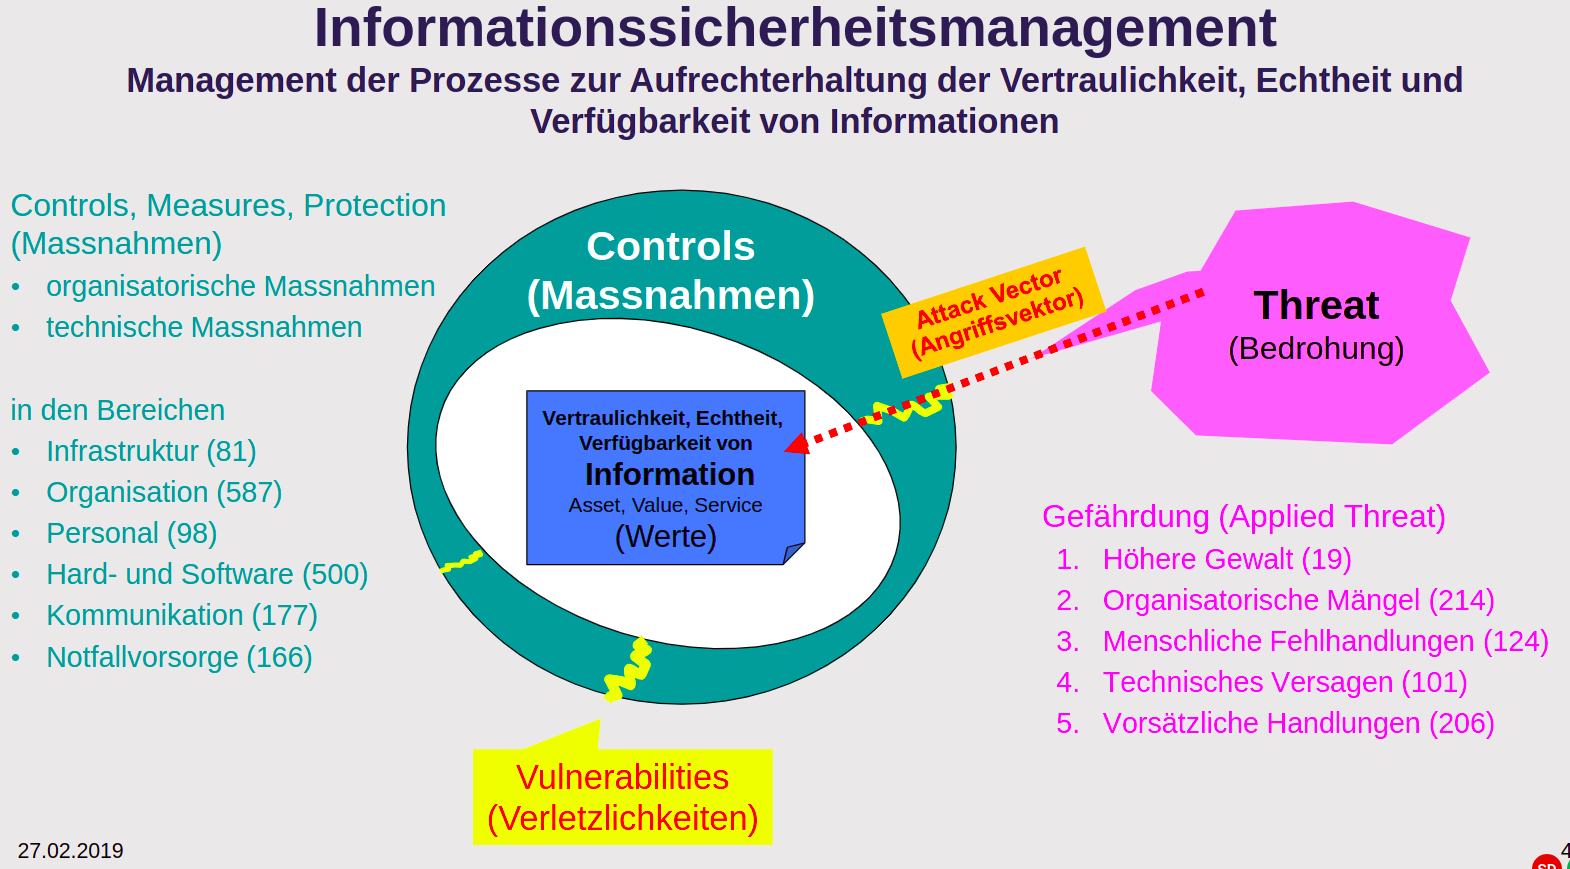
\includegraphics[width=1.0\linewidth]{images/Informationssicherheitsmanagement}
	\caption{Modell Informationssicherheitsmanagement}
\end{figure}
\subsection{CIA}
\begin{description}
		\item[CIA: Confidentiality, Integrity, Availability] \hfill
		\begin{enumerate}
			\item Vertraulichkeit / Confidentiality
			\begin{itemize}
				\item Abhören der Daten: Eavesdropping, Sniffing, mitlesen der Daten
			\end{itemize}
			\item Echtheit / Integrity, Authencity
			\begin{itemize}
				\item Integrity: Echtheit der Meldung: Forge, Modify, Fake = verändern der Daten
				\item Authenticity: Echtheit des Senders: Spoof, Hijack, Masquerade, Man In The Middle
			\end{itemize}
			\item Verfügbarkeit / Availability
			\begin{itemize}
				\item Flooding, DoS
			\end{itemize}
			\item Zusätzliche Eigenschaften sind Authentizität, Verantwortlichkeit, Nicht Abstreitbarkeit (non repudiation) und Zuverlässigkeit
		\end{enumerate}	
\end{description}

\subsection{Risikomanagement}
\begin{enumerate}
	\item Risikoidentifikation: Möglichst vollständige Erfassung der Gefahrenquellen und der möglichen Konsequenzen
	\item Risikobewertung: Beurteilung der Risiken unter der Berücksichtigung von Eintrittswahrscheinlichkeit und Schadensausmass (Risikotabelle). Dabei muss auch immer der Aufwand und Ertrag berücksichtigt werden.
	\item Risikobewältigung: Mit Hilfe der gewonnen Informationen Massnahmen einleiten um die Risiken zu minimieren oder gar zu eliminieren.
\end{enumerate}

\subsubsection{Risikoanalyse}
Die meisten IT-Gesamtsysteme enthalten ähnliche Komponenten (Server, Clients, Serverraum, E-Mail...). Man kann in erster Näherung immer von ähnlichen Gefährdungen und Eintrittswahrscheinlichkeiten ausgehen, d.h. es ist in den meisten Fällen keine klassische Risikoanalyse nötig. Ferner gibt es Standard-Sicherheitsmassnahmen, welche generell sinnvoll sind. Zur Risikoanalyse gehört nur die Identifikation und Bewertung.

\subsubsection{Risiko}
Ist die Möglichkeit, dass eine Bedrohung eine Schwachstelle
ausnutzen und dadurch der Institution Schaden zufügen könnte. Das Risiko ist eine Kombination aus Wahrscheinlichkeit eines Ereignisses und dessen Auswirkung. Das Risiko kann wie folgt berechnet werden:
\begin{itemize}
	\item Risiko = Eintrittswahrscheinlichkeit (1-5) $\cdot$ Schadenspotential (1-5)
\end{itemize}
\subsubsection{Risikomatrix}
Die Risikomatrix veranschaulicht die Werte der Risikoanalyse auf zwei Achsen. In Zellen werden die Referenzen auf die Risikobeschreibung notiert. 
\begin{figure}[h]
	\centering
	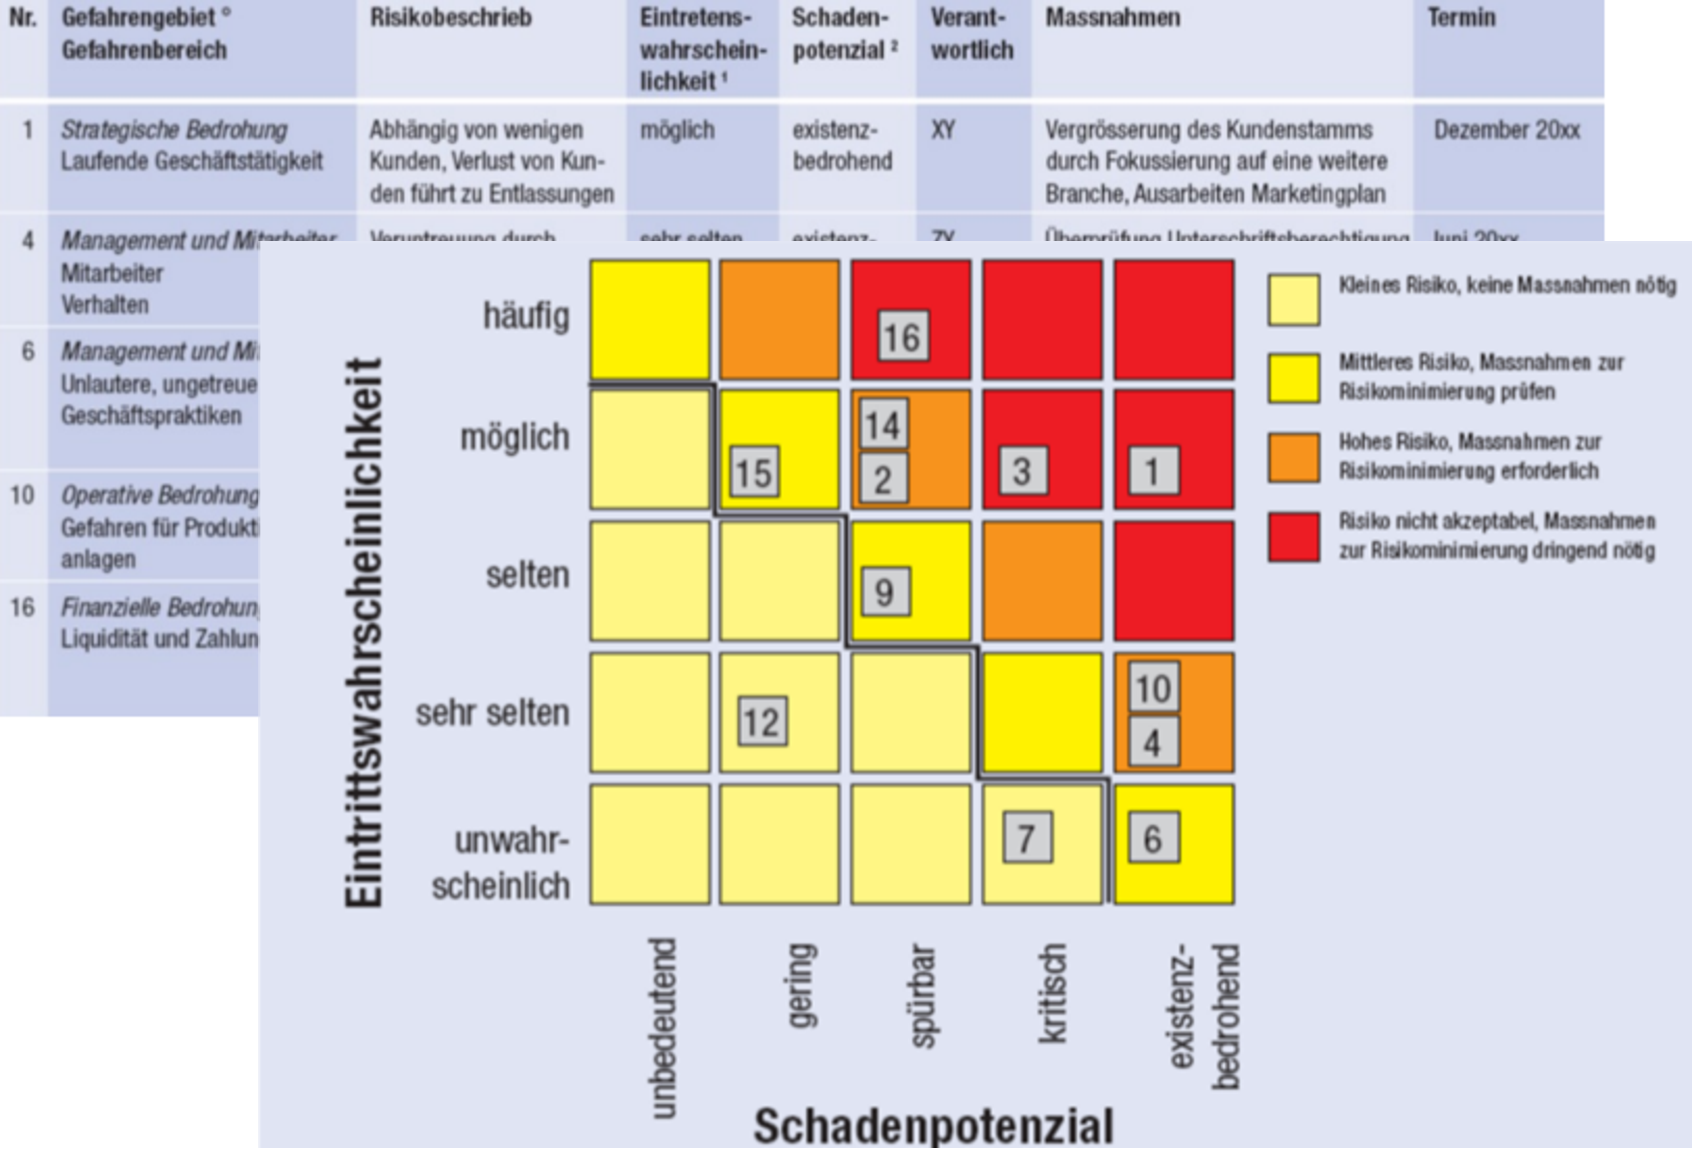
\includegraphics[width=0.8\linewidth]{images/risikomatrix}
	\caption{Risikotabelle mit Risikomatrix}
\end{figure}
\begin{enumerate}
	\item Eintrittswahrscheinlichkeit (Y-Achse)
	\begin{itemize}
		\item sehr selten (1)
		\item selten (2)
		\item gelegentlich (3)
		\item häufig (4)
		\item sehr häufig (5)
	\end{itemize}
	\item Schadenspotential (X-Achse)
	\begin{itemize}
		\item unbedeutend (1)
		\item gering (2)
		\item spürbar (3)
		\item kritisch (4)
		\item existenzbedrohend (5)
	\end{itemize}
\end{enumerate}

\section{Standardisierung}
Ein Standard ist eine einheitliche, weithin anerkannte und meist auch angewandte Art, etwas herzustellen oder durchzuführen, die sich gegenüber anderen Arten durchgesetzt hat.

\begin{description}
	\item[De-Facto Standard] Ein De-Facto Standard ist ein hersteller Spezifischer Standard, der sich über die Jahre  durchgesetzt hat und hauptsächlich verwendet wird. (ASCII, ECMA, PDF, SQL)
\end{description}

\subsection{ISO 27000}
\begin{itemize}
	\item Internationaler Standard, wobei 75\% der an der Abstimmung beteiligten Nationen dem Standard zustimmen müssen. Eine positive Verabschiedung eines Standard dauert meist 2-4 Jahre
	\item Beinhaltet mehrere Sub Standards zum Thema ISMS (Information Security Management Systems)
	\item Wird von ISO herausgegeben
	\item Kostet ca. 138CHF und ist somit der teuerste Standard
	\item Ist der kürzeste Standard (27 Seiten)
	\item ISO 27001 beschreibt die Norm 
	\item ISO 27002 beschreibt die Umsetzung der Norm (umfangreicher wie 27001)
	\item ISO 27005 beschreibt die Risikoanalyse
\end{itemize}

\subsubsection{PDCA: Plan, Do, Check, Act}
Das Qualitätsmanagement sollte als Kreislauf der folgenden vier Punkte organisiert werden. Es ist die Aufgabe des Management diesen Kreislauf von Walter Edwards Deming umzusetzen. Der Deming Cycle ist teilt des ISO 27001
\begin{enumerate}
	\item Plan: define goals, get an overview, Ziele, Ressourcen, potentielle Fehler, Anleitungen festlegen
	\item Do: impelement, operate, sorge für die Durchführung der Planung
	\item Check: monitor, review, Überwache den Fortschritt der Arbeiten.
	\item Act: Maintain, improve, Fehleranalyse, Evaluation von Lösungsmöglichkeiten, Fehlerbehebung.
\end{enumerate}

\subsubsection{Keywords}
\begin{enumerate}
	\item MUST, REQUIRED, SHALL: müssen unbedingt umgesetzt werden
	\item MUST NOT, SHALL NOT: dürfen auf keinen Fall umgesetzt werden
	\item SHOULD, RECOMMENDED: Kann unter Umständen weggelassen werden, gilt aber als besonders angemessen und sollte deshalb umgesetzt werden.
	\item SHOULD NOT, NOT RECOMMENDED: Unter gewissen Umständen akzeptierbar. Es sollte aber nicht vorkommen.
	\item MAY, OPTIONAL: optional
\end{enumerate}

\subsection{ITIL: IT Infrastructure Library}
\begin{itemize}
	\item Lehnt an ISO 27001 an, ist jedoch für kleinere Unternehmen ausgelegt.
	\item ITIL konzentriert sich auf IT Service Management
\end{itemize}

\subsection{BSI: Bundesamt für Sicherheit in der Informatik}
\begin{itemize}
	\item Das BSI ist dem deutschen Innenministerium zugeordnet und gibt unter anderen Kompetenzen Tipps für den IT Grundschutz
	\item Ein offizielles BSI Zertifikat mit Auditor kostet um die 2500 Euro
	\item Die BSI IT-Grundschutz Unterlagen sind gratis verfügbar
	\item Ist kein internationaler Standard und daher nicht von internationaler Gültigkeit
	\item Beinhaltet teilweise veraltete Bausteine
	\item BSI Gefährdungskatalog
	\begin{itemize}
		\item G1: Höhere Gewalt
		\item G2: Organisatorische Mängel: Fehlende Regelungen (Passwort/PIN, Beaufsichtigung der Geräte, Updating, Patching, Malware Detection), Unzureichende Ausbildung
		\item G3: Menschliche Fehlhandlungen: Regelungen werden nicht eingehalten, Blindes Vertrauen, Bedienungsfehler
		\item G4: Technisches Versagen: Fehler in Schutzmassnahmen, unzureichende Verschlüsselung, Versteckte Funktionen.
		\item G5: Vorsätzliche Handlungen
	\end{itemize}
	\item BSI Massnahmenkatalog
	\begin{itemize}
		\item M1: Infrastruktur
		\item M2: Organisation
		\item M3: Personal
		\item M4: Hardware / Software
		\item M5: Kommunikation (Netze)
		\item M6: Notfallvorsorge
	\end{itemize}
\end{itemize}

\subsection{NIST: National Institute of Standards and Technology}
NIST ist das nationale Standardisierungsinstitut der USA.
\begin{description}
	\item[NVD: National Vulnerability Database (früher CVE: Common Vulnerabilities and Exposures)] \hfill \\
	ist eine Sammlung von Sicherheitslücken der NIST. Jede Lücke hat eine eindeutige ID in diesem Katalog. Es existiert eine Open Source Alternative der Black Hat Konferenz namens OSVDB.
	\item[CPE: Common Platform Enumeration Dictionary] \hfill \\ Dient einer einheitlichen Namensgebung der betroffenen Produkte und Hardware.
	\item[CWE: Common Weakness Enumeration] \hfill \\ Dient einer einheitlichen Namensgebung der Sicherheitslücken
	\item[CVSS: Common Vulnerability Scoring System] \hfill \\ Dient der Gewichtung der Lücken. (0-10)	
\end{description}

\subsubsection{NIST Glossar of Key Information Security Terms}
\begin{itemize}
	\item Beinhaltet alle Begriffe die wichtig sind um die NIST Publikationen zu verstehen
	\item Wird vom National Institute for Standards and Technologies herausgegeben
	\item Ist gratis
	\item 222 Seiten
\end{itemize}

\subsection{RFC 4949 (Request for Comments)}
\begin{itemize}
	\item Open Source Standard und wird von der IETF (Internet Engineering Task Force) herausgegeben
	\item Beschreibt weit mehr als nur Security Begriffe. Ist viel umfangreicher, technischer und detaillierter als die ISO Standards.
	\item Ist gratis verfügbar
	\item Bei der IETF läuft der Standardisierungsprozess meist am schnellsten ab
	\item 365 Seiten
\end{itemize}

\subsection{ANSI: American National Standards Institution}
\begin{itemize}
	\item Können nur zwei Vertreter pro Firma Mitglied sein
	\item Ist nicht gratis verfügbar
\end{itemize}

\subsection{IEEE: Institute of Electrical and Electronics Engineers}
\begin{itemize}
	\item IEEE ist der weltweit grösste Berufsverband von Ingenieuren auf der ganzen Welt. 
	\item In den Standardisierungsgremien kann jedermann teilnehmen. 
	\item Stimmberechtigt sind alle die an genügend vielen Sitzungen teilgenommen haben.
	\item Dieser Standard ist nicht kostenlos erhältlich
\end{itemize}

\subsection{OWASP: Open Web Application Security Project}
Gibt Empfehlungen für den sicheren Bau von Webapplikationen heraus. OWASP gibt eine Liste von Web Schwachstellen heraus, welche nach ihrem Risiko geordnet ist.

\subsection{CERT: Computer Emergency Response Team}
Das CERT wurde 1988 von der DARPA (Defense Advanced Research Project Agency) in den USA gegründet und hat die Aufgabe Informationen über Sicherheitsaspekte und -vorfälle im Internet zu sammeln und zu veröffentlichen.

\subsection{PCI DSS: Payment Card Industry Data Security Standard}
\begin{itemize}
	\item PCI DSS ist ein Standard für den Zahlungsverkehr mit Kreditkarten
\end{itemize}

\section{Gefährdungen}
\subsection{Motivation zum Cracken}
Sortiert nach steigendem Know-How
\begin{enumerate}
	\item Langeweile = Jedermann / Script Kiddies
	\item Persönliche Profilierung = IT Freak
	\item Persönlicher Gewinn = Auftrags Cracker
	\item Politisches Interesse = Hacktivismus
	\item Nationales Interesse = Geheimdienst / Wirtschaftsspionage
\end{enumerate}

\subsection{Angriffsarten}
\begin{description}
	\item[Clickjacking] \hfill \\ Unsichtbares Overlay über Steuerelemente. Der User wird animiert auf eine bestimmte Stelle zu klicken und löst damit unbewusst eine schädliche Aktion aus.
	\item[Drive By Downloads] \hfill \\ Hier wird beim Download einer vermeidlich gutartigen Datei etwas schlechtes mit herunter geladen. 
	\item[Inside Out Attacke] \hfill \\ Beim Aufruf einer Webseite wird wird Code mitgeliefert, der z.B den Heimrouter um konfiguriert und somit den Zugriff von Ausserhalb ermöglicht.
	\item[MMI: Man Machine Interface] \hfill \\ Factory Reset via QR Code
	\item[Botnets] \hfill \\ Mehrere infizierte Computer die via Remote gesteuert werden und für das Versenden von Spam oder DDOS Attacken genutzt werden.
	\item[Phishing] \hfill \\ Locken von Benutzern auf vermeidlich ähnliche Seite wie das Original, wobei vertrauliche Informationen abgegriffen werden.
	\item[Spear Phishing] \hfill \\ Gezielter Angriff auf ausgewählte Personen, mittels Social Engineering
	\item[Man in the Middle / Janusangriff] \hfill \\ ARP Spoofing, DNS Cache Poisoning, Roque WLAN Hotspots. Ein Angreifer lässt den Datenverkehr zweier Kommunikationspartner über sich laufen und kann damit die komplette (unverschlüsselte) Kommunikation mitlesen.
	\item[Ransomware] \hfill \\ Verschlüsselt die Daten auf einem Gerät und fordert für die Entschlüsselung Lösegeld
\end{description}

\subsection{WWW: World Wide Web}
\begin{description}
	\item[Surface Web / Lightweb:] Indexiert und per Suchmaschine auffindbare Informationen
	\item[Deep Web:] Beschreibt den versteckten, nicht indexierten Teil des World Wide Webs
	\item[Dark Web:] Nur über Tor erreichbar
\end{description}


\section{Rechtslage}
\begin{itemize}
	\item Typische Vergehen sind:
	\begin{itemize}
		\item Hacken: Unbefugtes Eindringen in fremde Netzwerke und Daten
		\item Urheberrechts-Verstösse: Software Piraterie
		\item Verbreitung von Kinderpornografie
		\item Betrug, Geldwäsche, Vorbereitung terroristischer Akte
	\end{itemize}
	\item wobei man zwischen Übertretungen, Vergehen und Verbrechen unterscheidet.
	\item Schweizer Meldestellen sind MELANIE für Sicherheitszwischenfälle und KOBIK für koordinierte Bekämpfung der Internet Kriminalität
\end{itemize}

\paragraph{Unbefugte Datenbeschaffung (Art. 143)}
Wer sich unbefugt Daten beschafft, die gegen unbefugten Zugriff besonders gesichert sind, muss mit einer Freiheitsstrafe bis zu fünf Jahren oder einer Geldstrafe rechnen.

\paragraph{Unbefugtes Eindringen in ein Datenverarbeitungssystem (Art. 143bis)}
Wer sich Zugriff in ein besonders gesichertes Datenverarbeitungssystem verschafft, wird, auf Antrag,  mit einer Freiheitsstrafe bis zu drei Jahren oder einer Geldstrafe bestraft. (Hacking Tatbestand)

\paragraph{Verbreiten von Passwörter, Programme und andere Daten (Art. 143bis)}
Wer Passwörter, Programme oder andere Daten verbreitet, von denen er annehmen muss, dass sie für illegale Zwecke verwendet werden können, wird mit einer Freiheitsstrafe von bis zu drei Jahren oder einer Geldstrafe bestraft.

\paragraph{Datenschädigung (Art. 144bis Ziffer 1)}
Wer unbefugt elektronisch gespeicherte oder übermittelte Daten verändert, löscht, oder unbrauchbar macht, wird auf Antrag mit einer Freiheitsstrafe von bis zu drei Jahren oder einer Geldstrafe bestraft. In Härtefällen kann sogar auf eine Freiheitsstrafe von bis zu 5 Jahren entschieden werden.

\paragraph{Datenschädigung (Art. 144bis Ziffer 2)}
Wer Programme gemäss Ziffer 1 (Viren etc.) herstellt, einführt, in Verkehr bringt, anpreist, anbietet oder sonst wie zugänglich macht oder zu ihrer Herstellung Anleitung gibt, wird mit einer Freiheitsstrafe bis zu drei Jahren oder einer Geldstrafe bestraft. In Härtefällen (gewerbsmässige Handlung) kann sogar auf eine Freiheitsstrafe von bis zu 5 Jahren entschieden werden. (Virentatbestand)

\paragraph{Computerbetrug / Betrügerischer Missbrauch einer Datenverarbeitungsanlage (Art. 147 StGB)}
Wer sich oder einen anderen unrechtmässig bereichert und daher eine Vermögensverschiebung zum Schaden eines Zweiten herbeiführt, wird mit einer Freiheitsstrafe bis zu fünf Jahren oder einer Geldstrafe bestraft. In Härtefällen (gewerbsmässige Handlung) kann sogar auf eine Freiheitsstrafe von bis zu 10 Jahren oder einer Geldstrafe von min. 90 Tagessätzen entschieden werden.

\paragraph{Datensicherheit (Art. 7)}
Personendaten müssen durch angemessene technische und organisatorische Massnahmen gegen unbefugtes Bearbeiten geschützt werden.

\paragraph{Allgemeine Massnahmen (Art. 8)}
Wer als Privatperson Personendaten bearbeitet oder ein Datenkommunikationsnetz zur Verfügung stellt, sorgt für die Vertraulichkeit, die Verfügbarkeit und die Richtigkeit der Daten, um einen angemessenen Datenschutz zu gewährleisten. Insbesondere schützt er die Systeme gegen folgende Risiken:
\begin{itemize}
	\item unbefugte oder zufällige Vernichtung
	\item zufälligen Verlust
	\item technische Fehler
	\item Fälschung, Diebstahl oder widerrechtliche Verwendung
	\item unbefugtes Ändern, Kopieren, Zugreifen oder andere unbefugte Bearbeitungen
\end{itemize}


\subsection{Beispiele}
\begin{description}
	\item[World Economic Forum Hack] \hfill \\ Die Kreditkarteninformationen, Mail Adressen und Telefonnummern von mehreren bekannten Politiker wurden von den Servern des WEF's entfernt. Dabei wurde die Confidentiality verletzt. Eine Person wurde verhaftet, man konnte sie aber nicht verurteilen da der Server nicht speziell gesichert war.
	\item[Viren Quellcode verteilen] \hfill \\ Ein EDV Experte verteilte den Quellcode für Computerviren und wurde zu 5000  CHF Busse sowie 2 Monaten Gefängnis verurteilt. 
\end{description}

\section{Massnahmen}
\begin{enumerate}
	\item Organisieren (Übersicht schaffen, Klassifizieren, Ziele festlegen, Risikomanagement)
	\item Zugriff kontrollieren (Zugangsschutz, IAM, Firewalls, Biometrische Scans)
	\item Massnahmen kombinieren
	\begin{description}
		\item[Multilevel Security] Sicherheit auf mehreren OSI-Layer
		\item[In Depth Security] Produkte von unterschiedlichen Hersteller einsetzen
	\end{description}
	\item Umsetzung kontrollieren (Penetration Tests, Reviews, Audits, Zertifizierungen, Honey Pots)
	\item Fehler korrigieren
\end{enumerate}

\subsection{Filterstrategien}
\begin{description}
	\item[Principle of Least Priviledge] Nur zulassen, was unbedingt nötigt ist
	\item[Same Origin Policy] \hfill \\
	Nur zulassen, was von einem bestimmten Bereich kommt (z.B. Cookie setzen via JavaScript)
	\item[Sandbox] Aktionen nur innerhalb eines bestimmten Bereichs zulassen
	\item[Opt Out, Black List] Alles erlauben, was nicht ausdrücklich verboten ist
	\item[Opt In, White List] Alles verbieten, was nicht ausdrücklich erlaubt ist
	\item[Vier Augen Prinzip] Nur zulassen was mindestens zwei Personen gutheissen
\end{description}

\subsection{JUST Culture (Justice) }
Regeln können auch missachtet werden. Es geht immer um den gesunden Menschenverstand.
\begin{itemize}
	\item Menschliche Fehler: Müssen gemeldet werden. Werden aber toleriert
	\item Risikobehaftetes Verhalten: Muss gecoached werden
	\item Rücksichtloses Verhalten: Muss bestraft werden
\end{itemize}

\section{Kryptographie}
\subsection{Begriffe}
\begin{description}
	\item[Kryptologie] Ist die Lehre der Verschlüsselungs- und Entschlüsselungstechnik.
	\item[Kryptographie] \hfill \\ Ist die Wissenschaft von der Ver- und Entschlüsselung von Daten mit Hilfe mathematischer Verfahren.
	\item[Kryptoanalyse] Ist die Lehre des Knackens von kryptographisch abgesicherter Meldungen.
	\item[Cipher] ist der verschlüsselte Text
	\item[Security by Obscurity] \hfill \\
	Die Sicherheit eines Systems beruht darauf, dass seine Funktionsweise geheim gehalten wird.
	\item[Forward Secrecy] \hfill \\
	Für jede Nachricht wird ein neuer Schlüssel verwendet. (Session Key) Zusätzlich wird jeder ''Session Key'' nach der erfolgreichen Übertragung gelöscht. Dies bietet zwei klare Vorteile: Angenommen die Nachrichten wurden z.B durch Vorratsdatenspeicherung aufgezeichnet und der private Schlüssel wurde geknackt oder musste durch einen Gerichtsbeschluss herausgegeben werden. In diesem Fall ist 1) der Schlüssel gar nicht mehr vorhanden (er wurde nach der Übertragung gelöscht) und 2) kann im schlimmsten Fall nur eine einzige Nachricht und nicht die Kommunikation über mehrere Jahre entschlüsselt werden.
	\item[KDF: Key Derivation Function] \hfill \\
	Mittels Key Derivation können ausgehend von einem privaten Schlüssel mehrere neue private Sub-Schlüssel berechnet werden. (Session Keys) Eine Key Derivation Function ist mit einer Hash Funktion zu vergleichen. Man übergibt der Funktion den ursprünglichen Schlüssel und einen Subkey Index und bekommt einen neuen Subkey. Wie bei einer Hashfunktion kann man nicht auf den ursprünglichen Schlüssel schliessen.
	\item[Plausible Deniability] \hfill \\
	Bei Plausible Deniability geht es darum, den Ursprung einer Sache so zu verbergen, dass dieser nicht nachgewiesen werden kann.
\end{description}

\subsection{Design Aspekte}
\begin{enumerate}
	\item Der Algorithmus soll offen sein, der Schlüssel jedoch geheim.  (Kerckhoffs-Prinzip)
	\item Wenn man im Klartext ein Bit ändert, sollen möglichst viele Bits im Schlüssel ändern (Shannon Prinzipien)
	\item Der beste Angriff sollte maximal so gut sein wie ein Brute Force Angriff
	\item Die Cipher sollte möglichst gut einer Zufallsfolge gleichen
\end{enumerate}

\subsection{Informationsgehalt}
Der Informationsgehalt eines Zeichens entspricht dem negierten Zweierlogarithmus des Wahrscheinlichkeit eines Zeichens. Je kleiner also die Wahrscheinlichkeit des Auftretens eines Zeichens ist, desto grösser ist der Informationsgehalt. 
\begin{align}
I_i(x_i)=-\log_2(p_i)
\end{align}	
	
\paragraph{Redundanz}
 Differenz zwischen maximal möglichem und mittlerem Informationsgehalt

\subsection{Entropie}
Die Entropie ist der durchschnittlicher Informationsgehalt über alle Zeichen. Die Entropie ist maximal wenn alle Zeichen gleich wahrscheinlich auftreten. Bei einer binären Quelle ist die maximale Entropie = 1, nämlich genau dann wenn es gleich viele 0en und 1sen gibt. Deutsche und englische Text haben eine Entropie von 4.7Bit/Zeichen Die Entropie wird in Bit pro Zeichen gemessen.

\begin{align}
\begin{split}
Entropie &= -  \sum_{i=0}^n (p_i \cdot \log_2(p_i)) \\
Entropie_{max} &= log_2(n)
\end{split}
\end{align}
wobei
\begin{itemize}[label=]
	\item $p_i$ = Wahrscheinlichkeit eines Zeichens
	\item n=Anzahl Zeichen im Alphabet
\end{itemize}



\subsection{Steganographie}
Die Steganografie beschäftigt sich mit dem unauffälligen Verstecken von Nachrichten innerhalb von digitalen Objekten, beispielsweise von Texten, Grafiken, Videos oder Fotos. Die Steganographie hat nichts mit Kryptographie zu tun, das sie nur verdeckt, aber nicht verschlüsselt.

\subsubsection{Watermarking}
Watermarking ist eine spezielle Methode der Steganographie. Beim Watermarking werden unauffällige Hinweise hinterlegt, um den Urheber einer Datei zu bestätigen. Watermarking existiert auch in der Festplattenverschlüsselung, wobei man dort beweisen möchte, dass sich eine bestimmte Datei auf einer verschlüsselten Festplatte befindet. (z.B Kinderpornographie)

\subsection{Transpositionsverfahren}
Die Transposition war ein erster Ansatz der Verschlüsselung. Bei den Transpositionsverfahren werden die Buchstaben des Klartextes in ihren Positionen
vertauscht (umsortiert). Ein Beispiel ist der Skytale von Sparta. Dabei wurde ein Papier Streifen um einen Zylinder gewickelt, wobei die Nachricht nur mit einem Zylinder gleicher Dicke gelesen werden konnte.

\subsection{Substitutionsverfahren}
Beim Substitutsionsverfahren wird jedes Zeichen des Klartextes durch ein anderes ersetzt. (Caesar, Vigenere)

\subsection{Monoalphabetic Substitution Cipher}
Es wird nur ein einziges fixes Alphabet zur Verschlüsselung/Substitution verwendet.

\subsubsection{Caesar Code}
Der Caesar Code ist eine monoalphabetische Verschlüsselung, mit $26$ möglichen Schlüssel. (26 Buchstaben im Alphabet) Als Schlüssel dient eine feste Zahl, die bestimmt, mit welchem Zeichen ein Klartextzeichen ersetzt wird. Caesar Code kann mit der Häufigkeitsverteilung der Buchstaben gebrochen werden. 

\subsection{Polyalphabetic Substitution Cipher}
Hierbei werden mehreren Verschlüsselungsalphabete verwendet. Genauer gesagt bestimmt der Schlüssel um wie viele Zeichen sich das Klartextzeichen verschiebt. Dabei wird jedes Klartextzeichen um unterschiedlich viele Zeichen verschoben.

\subsubsection{Vigenere Code}
Beim Vigenere Code bestimmt ein geheimer Schlüssel um wie viele Zeichen ein Klartext Zeichen verschoben wird. Dabei wird die Buchstabennummer des Schlüssels verwendet (beginnend bei A = 0). Es gibt ein vorberechnetes Vigenere Quadrat mit dessen Hilfe das Ver-, und Entschlüsseln relativ einfach von statten geht. Vigenere kann sehr einfach mittels Autokorrelation geknackt werden. Die periodisch wiederkehrenden Maximalwerte deuten auf die Schlüssellänge des Vigenere Codes. (Ausnahme: One-Time-Pad). Der Vigenere Code ist ein polyalphabetisches Substitutionsverfahren. Wird der Klartext mit zwei Schlüssel unterschiedlicher Länge verschlüsselt entspricht die neue Schlüssellänge dem kgV() der beiden Schlüssel. Bei Vigenere gibt es $26^n$ mögliche Schlüssel

\subsection{Histogramm}
In einem Histogramm wird der prozentuale Anteil der Auftretungshäufigkeit eines Zeichens dargestellt.

\subsection{Autokorrelation}
Bei der Autokorrelation wird ein Text mit verschobenen Kopien desselben Textes verglichen. Dabei werden jeweils die übereinstimmenden Zeichen ermittelt. Kongruente Werte werden dann in einem Diagramm dargestellt, wobei auf der Y-Achse die Anzahl der übereinstimmende Zeichen (Hits) und auf der X-Achse die Grösse der Verschiebung dargestellt wird.
\begin{figure}[h]
	\centering
	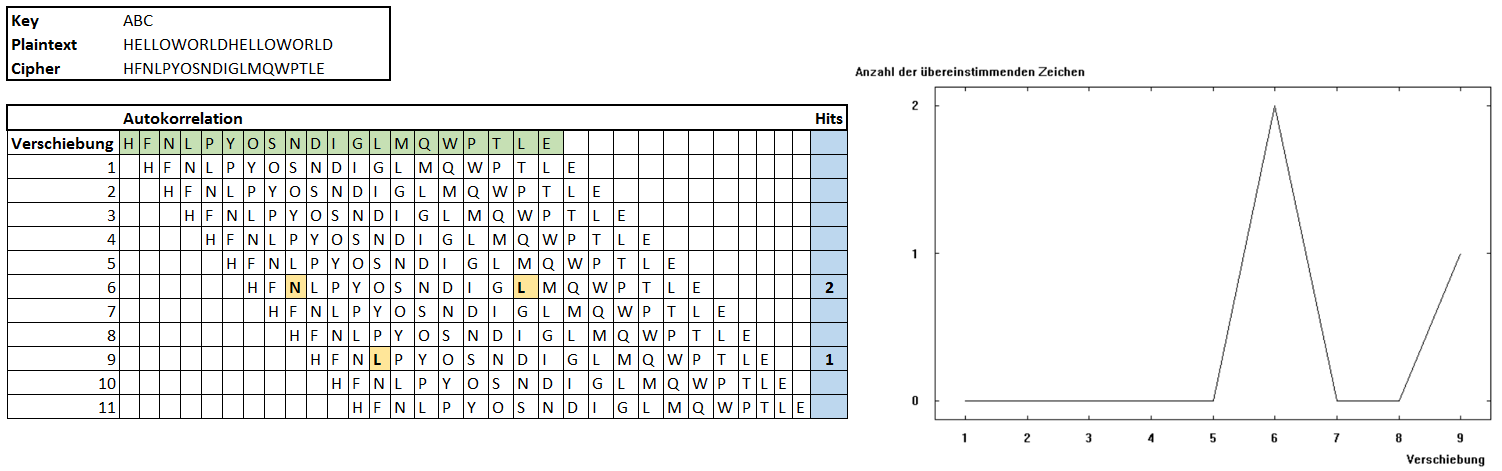
\includegraphics[width=0.8\linewidth]{images/autokorrelation}
	\caption{Beispiel: Autokorrelation}
\end{figure}

\subsection{OTP: One-Time-Pad / Vernam Chiffre}
Beim One Time Pad ist der Schlüssel mindestens so lang wie die Nachricht selbst. Ebenfalls ist der Schlüssel zufällig und wird nur genau einmal verwendet. Wird es richtig angewendet, kann es nachweislich nicht gebrochen werden. Bei der Vernam Chiffre wird der Klartext und der Schlüssel mittels XOR zur Chiffre vereint. Es gibt genau so viele Schlüssel wie es Cipher gibt. 

\subsection{Schlüssellänge}
Wird die Länge eines Schlüssels um ein Bit erhöht, wird die Sicherheit des Systems exponentiell vergrössert und der Informationsgehalt nimmt um ein Bit zu. Falls die Schlüssellänge von x auf y erhöht wird, so gibt es $2^{y-x}$ mögliche Schlüssel mehr.

\begin{tabular}{|l|l|l|}
	\hline Symmetrisch & RSA & ECC \\ 
	\hline 80  & 1024  & 163 \\ 
	\hline 112 & 2048  & 233 \\ 
	\hline 128 & 3072  & 283 \\ 
	\hline 192 & 7680  & 409 \\ 
	\hline 256 & 15360 & 571 \\ 
	\hline 
\end{tabular} 

\[
	\text{Anzahl Schlüssel} = 2^{\text{Anzahl Bit}} 
\]

\subsection{Angriffe}
\begin{description}
	\item[Ciphertext-Only Attack] \hfill \\
	Es stehen nur die abgefangenen Cipher zur Verfügung.
	\item[Known-Plaintext Attack] \hfill \\
	Es stehen bekannte Klartext-Cipher Paare zur Verfügung. Hilfreich zur Schlüsselermittlung sind unter anderem verschlüsselte Anfangs- und Endphrasen. (z.B ''Heil Hiltler'' oder ''Mit freundlichen Grüssen'') 
	\item[Chosen-Plaintext Attack] \hfill \\
	Hierbei kann ein Angreifer einem System beliebige Klartexte übergeben und anschliessend die resultierenden Ciphers analysieren und auf Veränderungen prüfen. Dies ist das minimale Angriffsszenario für asymmetrische Kryptosysteme.
\end{description}

\subsection{Symmetrische Kryptographie}
Symmetrische Verfahren verwenden sowohl für das Verschlüsseln, als auch für das Entschlüsseln, den gleichen 
Key. Der Schlüssel muss dabei absolut geheim gehalten werden. Das Problem bei symmetrischen Kryptographie ist der sichere Austausch des Schlüssels mit dem Empfänger. Da symmetrische Kryptographie im Vergleich zur asymmetrischen Variante performanter ist, wird sie insbesondere für die Verschlüsselung von Daten verwendet. Damit in einem Netz von n Teilnehmer alle miteinander kommunizieren können, sind $\frac{n(n-1)}{2}$ unterschiedliche Keys nötig. 

\subsection{Stream Cipher}
Bei Stromchiffren wird aus einem Schlüssel und einem Initialisierungsvektor zunächst ein Schlüsselstrom
generiert, das heisst eine pseudozufällige Folge von Bits, die dann auf die zu verschlüsselnde Nachricht bitweise XOR-addiert wird. Im Gegensatz zur Blockchiffre ist ein Stream Cipher nicht darauf angewiesen, dass sich erst genug zu verschlüsselnde Daten angesammelt haben, bis sie die Größe für einen fixen Block erreicht haben, sondern kann jedes Klartextzeichen sofort in ein chiffriertes Ausgabezeichen übersetzen. 

\subsubsection{PRNG: Pseudo Random Number Generator}
Ein PRNG ist ein deterministischer Zufallsgenerator der bei gleichen Ausgangsbedingungen immer das gleiche Ergebnis liefert. Dies ist nötig damit eine Bitfolge auch wieder entschlüsselt werden kann. Im Gegensatz dazu liefern nicht deterministische Zufallsgeneratoren auch bei gleichen Ausgangsbedingungen andere Werte. Man greift dazu oft auf physikalische Prozesse zurück (z.b Impulsschwankungen, thermisches Rauschen, radioaktiver Zerfall)

\subsubsection{LFSR: Linear Feedback Shift Register}
Ein LFSR wird bei Stream Cipher für die Generierung von Pseudozufallszahlen verwendet. Das Shift Register beinhaltet immer einen Initialwert, auch Seed genannt, von welchem fortlaufend bestimmte Bits mit dem Letzten der Folge XOR verknüpft werden. Ein PRNG mit n langen Shift Register kann maximal einen $2^n - 1$ langen Bit Stream erzeugen.

\begin{figure}[h]
\centering
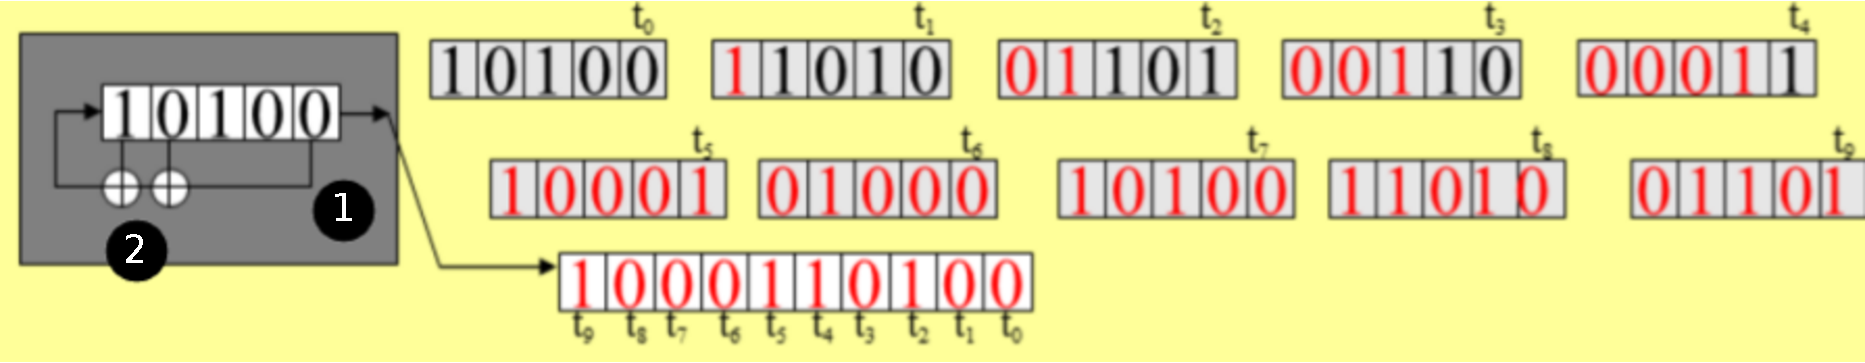
\includegraphics[width=0.7\linewidth]{images/lfsr}
\caption{LSFR: Linear Feedback Shift Register}
\end{figure}

\subsubsection{RC4: Ron's Code 4}
RC4 ist ein Stream Cipher mit variabler Länge des Schlüssels (zwischen 5 bis 256Bytes), das 1987 von Ron Rivest entwickelt wurde. RC4 wurde für WEP verwendet und gilt als gebrochen. Bei RC4 wird der Klartext Byte für Byte per XOR mit der Pseudozufallsfolge verknüpft. RC4 ist der einzige Stream Cipher seiner Reihe. (RC2, RC5, RC6 sind alles Block Codes). Verschlüsselt man einen Klartext zweimal mit RC4 kommt wieder der Klartext heraus. Ändert sich ein Zeichen im Cipher geht nur genau dieses Zeichen beim Entschlüsseln verloren.

\subsubsection{A5/1}
A5/1 ist ein Stream Cipher der für GSM verwendet wurde. Er verwendet Linear Feedback Shift Register. A5/1 wurde nur in Europa und den USA eingesetzt. Für Export Regionen wurde A5/2 entwickelt, der bewusst Schwachstellen implementiert hatte.

\subsection{Block Cipher}
Der Plaintext wird in Blöcke fixer grösse aufgeteilt und allenfalls gepadded. Die meisten Block Ciphers können 
sowohl im ECB als auch CBC Modus verwendet werden. 

\subsubsection{Block Cipher Modes}
\begin{description}
	\item[ECB: Electronic Codebook Mode] \hfill \\ Der Klassische Ansatz. Ein Klartextblock nach dem anderen wird unabhängig vom Rest verschlüsselt. Dabei führen im Gegensatz zu CBC/CFB gleiche Klartextblöcke immer auf die gleichen Ciphertextblöcke. Daher wird ECB für das Verschlüsseln grosser Datenmengen abgeraten, da periodische Muster im Cipher Text auftreten können. Wird im Cipher ein Zeichen verändert, geht beim Entschlüsseln nur genau der geänderte Block kaputt. Alle anderen Blöcke bleiben intakt.
	\item[CBC: Cipher Block Chaining] \hfill \\ Bei diesem Modus fliesst das Ergebnis der Verschlüsselung früherer Blöcke in die Verschlüsselung des aktuellen Blockes mit ein. Jeder Block des verschlüsselten Texters hängt also nicht nur vom zugehörigen Klartextblock sondern auch von allen vorherigen Klartextblöcken ab. Für den ersten Klartextblock wird zusätzlich ein Initialisierungsblock benötigt der zwischen Sender und Empfänger abgemacht werden muss. Zuerst wird der IV mit dem Klartext XOR verknüpft und danach das Resultat mit dem Schlüssel verschlüsselt. Ändert sich ein Zeichen im Cipher, ist nur der betreffende Block und der direkt Nachfolgende unlesbar.
	\begin{figure}[h!]
		\centering
		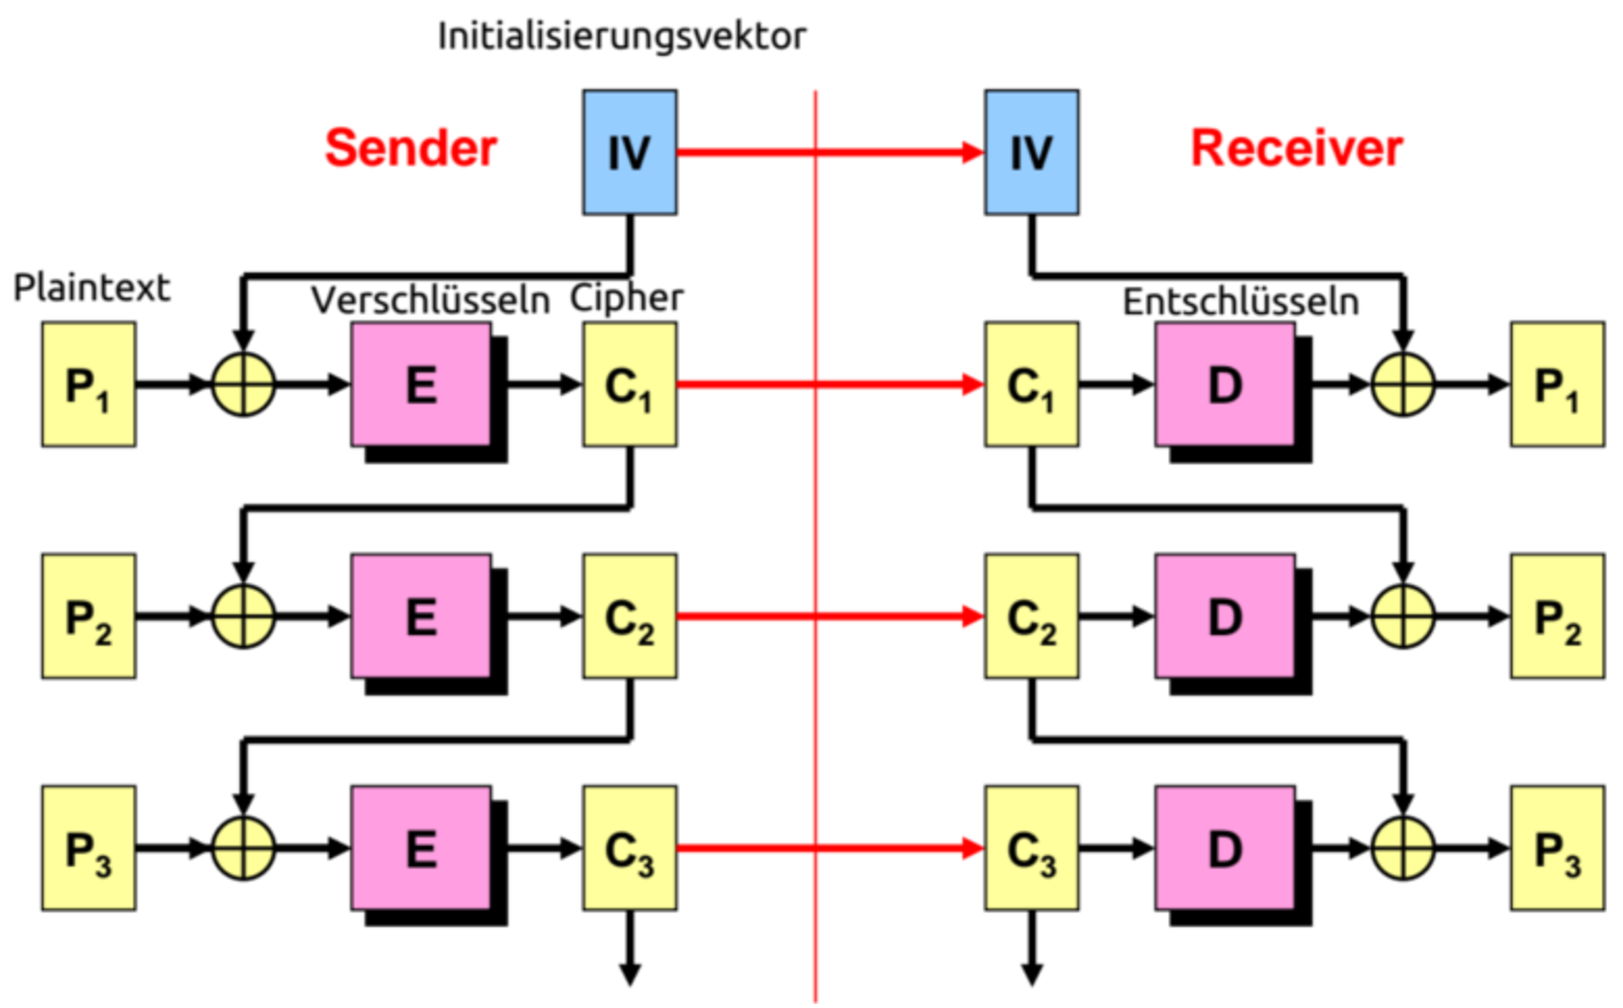
\includegraphics[width=0.5\linewidth]{images/cbc}
		\caption{CBC Mode}
	\end{figure}
	\item[CFB: Cipher Feedback] \hfill \\
	CFB ist eine Betriebsart, in der Blockchiffren als Stromchiffren betrieben werden, beispielsweise um damit Klartexte zu verschlüsseln, deren Länge kein Vielfaches der Blocklänge des Chiffrierverfahrens ist. Auch bei diesem Modus wird ein Initialisierungsvektor benötigt. Im Gegensatz zu CBC wir hier aber zuerst der IV mit dem Schlüssel verschlüsselt und das Resultat anschliessend mit dem Klartext XOR verknüpft. Die Abfolge von XOR und Verschlüsselung ist also genau umgekehrt.
	\item[CTR: Counter Mode] \hfill \\
	Hierbei wird eine Block Cipher in einen Stream Cipher konvertiert. Bei diesem Verfahren wird ein Key-Stream erzeugt, der die aufeinanderfolgenden Werte eines Zählers verschlüsselt. Als Zähler kann jede Funktion benutzt werden, die für einen längeren Zeitraum keine Wiederholung aufweist, so beispielsweise ein Zähler, der um den Wert 1 inkrementiert wird. Allerdings bieten so einfache Inkrementalzähler eine geringere Verschlüsselungssicherheit. 
\end{description}
	
\subsubsection{Padding}
\begin{description}
	\item[PKCS \#7 Padding] \hfill \\ Die Anzahl erforderlichen Padding Bytes wird als Binärzahl codiert und wird anschliessend als Padding verwendet. Es ist immer ein Padding Byte erforderlich, dass heisst es kann vorkommen das ein kompletter Block mit Padding aufgefüllt wird, da der vorhergehende Block genau gepasst hat.
	(AB CD EF GH | IJ KL 02 02)
	\item[ANSI X.923 Padding (CBC Mode bei DES)] \hfill \\ Padding mit Nullbytes, gefolgt von einem Byte, in welchem die Anzahl der Nachrichten Padding Bytes im letzten Block binär codiert ist. (z.B AA BB CC DD || 00 00 00 04) ACHTUNG: Im Crypttool werden die Datenbytes anstatt die Paddingbytes angegeben.
	\item[Null Padding (ECB bei DES)] \hfill \\ Hängt (sofern erforderlich) solange Null-Bytes an, bis die Blocklänge erreicht ist. Falls der Cipher mit 0en endet kann nicht eindeutig erkannt werden, wo das Padding anfängt und wo die Information endet. 
\end{description}

\subsubsection{DES: Data Encryption Standard}
DES ist ein symmetrisches Verschlüsselungsverfahren, das auf Klartextblöcken der Länge 64 Bits (= 8 Bytes) operiert und Blöcke mit verschlüsseltem Text der Länge 64 Bits erzeugt. Die Länge des Schlüssels beträgt ebenfalls 64 Bits; effektiv jedoch werden nur 56 Bits benutzt, da die jeweils niederwertigsten Bits (LSB rechts) der Schlüssel Bytes als Paritätsbits verwendet werden. (Total 8 Bit) So kann es vorkommen, dass sich ein Cipher mit zwei Schlüssel, welche sich nur in den Paritätsbits unterscheiden, entschlüsseln lässt. Mittels einer vollständigen Schlüsselraumsuche kann heutzutage eine mit DES verschlüsselte Nachricht in weniger als 25 Stunden geknackt werden. Beim Verschlüsseln mit dem DES-Verschlüsselungsverfahren wird für die Ver-/Entschlüsselung von jedem Schlüssel-Byte das niederwertigste Bit nicht verwendet, da es als Paritätsbit genutzt wird

\paragraph{Tripple DES} Bei 3DES wird jeder Datenblock mit einem ersten Schlüssel chiffriert, mit einem zweiten dechiffriert und mit einem dritten noch einmal verschlüsselt. Dieses Verfahren wird auch als EDE (Encrypt-Decrypt-Encrypt) bezeichnet. Sind alle drei Schlüssel gleich gewählt, sind die ersten zwei Durchläufe natürlich überflüssig. Das dreifache Ausführen der DES Operation führt zu einer Schlüssellänge von 168Bits wobei diese effektiv nur bei 112Bits liegt. Grund dafür ist der Meet-in-the-middle-Angriff.

\paragraph{MITM: Meet in the middle}
Der Meet in the Middle Angriff besagt, dass die effektive Schlüsselstärke von mehreren DES Iterationen schwächer ist als man annimmt. Dies kann am Beispiele von 2DES anschaulich erklärt werden. Dazu ist die folgende Formel mit den Umkehrfunktionen umzuformen.
\[
 Cypher = ENC_{k2}(ENC_{k1}(Plaintext))
\]
\[
 Plaintext = DEC_{k1}(DEC_{k2}(C)) 
\]
\[
\Rightarrow ENC_{k1}(P) = DEC_{k2}(C)
\]

Bei der Schlüssellänge nimmt man naiv an, dass die ein Angriff $2^{2n}$ Operationen benötigt, wie oben jedoch gezeigt benötigt man nur $2 \cdot 2^n$ rsp. $2^{n + 1}$


\subsubsection{AES: Advanced Encryption Standard}
AES wird heute standardmässig eingesetzt wenn etwas symmetrisch Verschlüsselt werden soll.
\begin{itemize}
	\item Block Cipher mit einer Blockgrösse von 128 Bit
	\item Es gibt drei Varianten von Schlüssellängen, welche sich nur in den Anzahl Runden unterscheiden
	\begin{enumerate}
		\item 128Bit: 10Runden
		\item 192Bit: 12Runden
		\item 256Bit: 14Runden
	\end{enumerate}
	\item AES verschlüsselt mit Software mit 200MBit/s und Hardware mit 1Gbit/s
	\item Gilt aktuell als sehr sicher
\end{itemize}

\subsubsection{Camellia}
Camellia verwendet die gleichen Parameter wie AES: eine Blockgröße von 128 Bit und Schlüssellängen von 128, 192 oder 256 Bit. Camellia wurde in Japan entwickelt und kann mit AES verglichen werden. Im Zweifelsfall sollte aber AES verwendet werden, da dieses Verfahren weiter verbreitet ist. 

\subsection{Asymmetrische Kryptographie}
Das Problem von symmetrischen Kryptographie ist das Verteilen der Keys über einen sicheren Kanal. Bei asymmetrischer Kryptographie hat ein jeder User ein Paar bestehend aus einem Public und einem Private Key. Der Public Key ist jedem zugänglich und wird über öffentliche Server verteilt. In einem Netz von n-Teilnehmer sind n Schlüsselpaare nötig, damit jeder mit jedem kommunizieren kann. Der private Schlüssel kennt nur der User selbst. Will nun Alice, Bob eine verschlüsselte Nachricht zustellen, verwendet sie Bobs öffentlicher Schlüssel und verschlüsselt damit ihre Nachricht. Die Nachricht kann nun nur noch mit dem privaten Schlüssel von Bob entschlüsselt werden.
Asymmetrische Kryptographie wird hauptsächlich für den Schlüsselaustausch und das Signieren von anderen Schlüsseln verwendet. 

\subsubsection{One Way Function}
Eine Ein-Weg Funktion ist einfach zu berechnen jedoch schwer das Inverse/Umkehrfunktion zu bilden. In einem erweiterten Sinn werden auch Funktionen so bezeichnet, zu denen bisher keine in angemessener Zeit praktisch ausführbare Umkehrung bekannt ist.

\subsubsection{Public Key Verfahren}
Das Public Key Verfahren wurde ursprünglich von den drei Kryptographen James H. Ellise, Clifford Cocks und Malcom Williamson erfunden. Die Drei arbeiteten  beim Britischen Geheimdienst (GCHQ), was dazu führte, dass aus Gründen der Geheimhaltung das erste asymmetrische Kryptosystem nicht veröffentlicht wurde.

\subsubsection{DH: Diffie-Hellman}
DH ist ein asynchrones Verfahren, welches dazu verwendet wird einen synchronen Key zu generieren. Die Idee 
hinter diesem Verfahren ist, dass die beiden Partner gemeinsam den geheimen Schlüssel generieren (Shared Master Secret), ohne ihn 
ganz übermitteln zu müssen. Bei TLS wird aus dem ephemeral Shared Master Secret das benötigte Pre-Master-Secret abgeleitet.

\paragraph{Vorgehen}
\begin{enumerate}
	\item One Way Function: $f(x) = g^x \text{ mod p}$
	\item Die Zahlen g und p sind öffentlich und können ungeschützt übertragen werden
	\item Alice und Bob einigen sich auf die Zahlen p und g
	\item Alice wählt eine zufällige Zahl a und sendet Bob den berechneten Wert gross A. $ A = g^a { mod(p)}$
	\item Bob wählt eine zufällige Zahl b und sendet Alice den berechneten Wert gross B. $ B = g^{b}{ mod(p)} $
	\item Beide können nun den geheimen Schlüssel K berechnen: $K= A^{b}{ mod(p)} $ rsp. $K= B^{a}{ mod(p)} $
\end{enumerate}

\subsubsection{EDH: Ephemeral Diffie-Helmman}
Die Verwendung von Ephemeral DH (flüchtige Keys) bietet Perfect Forward Secrecy und wird bei TLS verwendet. Dabei wird für jede TLS Sitzung neue Diffie-Hellman Parameter verwendet. (Siehe. PFS)

\subsubsection{Elgamal Kryptosystem}
Elgamal beruht auf dem mathematischen Problem des diskreten
Logarithmus, aufbauend auf der Idee des Diffie-Hellman-Algorithmus.

\subsubsection{RSA: Rivest, Shamir und Adleman}
Basiert darauf, dass es extrem schwierig ist eine grosse Zahl in seine Primfaktoren zu zerlegen. RSA wird unter anderem bei TLS verwendet wobei der TLS Client ein Pre-Master-Secret generiert und dies verschlüsselt an den TLS Server sendet.

\paragraph{Vorgehen}
\begin{enumerate}
	\item Zwei Primzahlen wählen und Produkt bilden: $n = p \cdot q$
	\item $\varphi(n) = (p - 1) \cdot (q - 1)$
	\item Beliebige Zahl a wählen, wobei a teilerfremd zu $\varphi(n)$ sein muss. ($ggt(\varphi(n), a) = 1$) \\ $\Rightarrow$ am besten eignen sich Primzahlen für a. (privater Schlüssel)
	\item Multiplikative Inverse b berechnen (öffentlicher Schlüssel) $a \cdot b = 1$ mod $\varphi(n)$ $\Rightarrow$ erweiterter Euklidischer Algorithmus
	\begin{enumerate}
		\item Modul: n (öffentlich)
		\item Öffentlicher Schlüssel: b
		\item Privater Schlüssel: a
	\end{enumerate}	
\end{enumerate}

\paragraph{Verschlüsseln}
\begin{enumerate}
	\item $\text{Wert}_\text{verschlüsselt} = (\text{Wert}_\text{unverschlüsselt})^{b} \cdot mod(n)$
\end{enumerate}

\paragraph{Entschlüsseln}
\begin{enumerate}
	\item $\text{Wert}_\text{unverschlüsselt} = (\text{Wert}_\text{verschlüsselt})^{a} \cdot mod(n)$
\end{enumerate}


\paragraph{Blöcke}
Um möglichst wenig Verschlüsselungen durchführen zu müssen, fast man in der Regel mehrere Zeichen zu Blöcken zusammen. 

\subsubsection{ECC: Elliptic Curve Cryptography}
Die Elliptische-Kurven-Kryptografie beruht darauf, dass es sehr aufwendig ist, diskrete Logarithmen auf elliptischen Kurven zu berechnen. Ihre Schlüsselzahlen entnehmen die elliptischen Kurven den Koordinaten von Punkten auf der Kurve. Bei einer Schlüssellänge von 160 Bit bietet ECC dieselbe Sicherheit wie das RSA-Verfahren mit einem 1024-Bit-Schlüssel. Dadurch ist dieses Verfahren schneller. Die bekannteste und meiste genutzte Kurve ist die Curve25519. Sie findet Anwendung in GPG, Sinal Protokoll und Tor. ($y^2 = x^3 + 48662x^2 + x$)

\begin{figure}[h!]
\centering
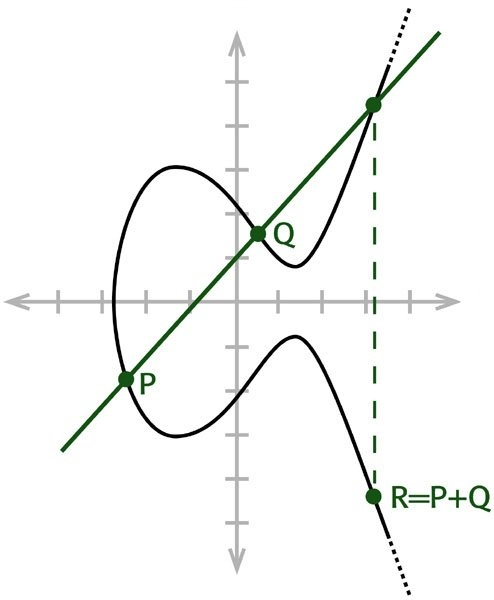
\includegraphics[width=0.2\linewidth]{images/ecc}
\caption{Elliptic Curve Cryptography}
\end{figure}


\subsubsection{Hybride Verschlüsselung}
Bei der Hybriden Verschlüsselung findet nur der Schlüsselaustausch asymmetrisch statt. Die eigentlichen Daten werden über ein effizientes, symmetrisches Verfahren verschlüsselt. 


\section{Digitale Signaturen}
\subsection{Signieren}
Beim Signieren geht immer um den CIA Punkt Integrity wobei folgende Punkte wichtig sind:
\paragraph{Integrität:} Eine Nachricht darf während der Übermittlung nicht verändert werden. Falls auch nur ein einziges Bit verändert wird, so kann dies der Nutzer der Daten anhand des Modification Detection Code erkennen.
\paragraph{Authentizität:} Mit Hilfe der Authentizität wird sichergestellt, dass eine Meldung tatsächlich von derjenigen Person
oder Institution stammt, welche sich als Absender ausgibt. Dies garantiert die Echtheit der Nachricht. 

\subsection{Hashing}
Eine Hashfunktion ist eine Abbildung, die eine große Eingabemenge auf eine kleinere Zielmenge (die Hashwerte) abbildet. To Hash heisst übersetzt zerhacken, verkleinern. Hash Funktionen sind immer One-Way Functions. Eine gute Hash Funktion erfüllt folgende vier Kriterien:
\begin{enumerate}
	\item Avalanche Effect: Ändert ein Bit, muss sich der ganze Hash komplett ändern
	\item Es muss sehr schwer sein, dass zwei Nachrichten auf den selben Hash führen. (Kollisions- Resistent) Zudem sollte es schwer sein ein zweite Nachricht zu finden, welches den gleichen Hash erzeugt.  (PreImage -Resistent)
	\item Hashes sollten nicht zu schnell sein, damit ein Durchprobieren unattraktiv ist.
	\item Der Speicherbedarf des Hash Wertes soll deutlich kleiner sein als der, der Nachricht. 
\end{enumerate}

\subsubsection{MDC: Modification Detection Code}
MDC ist eine kryptographische Hash-Funktion, die es erlaubt, Änderungen des Inhalts der Nachricht zu detektieren. Ein MDC-System generiert einen Bit-String, der an die verschlüsselten Nutzdaten angehängt wird. Die verschlüsselten Nutzdaten und der Bit-String werden entschlüsselt und anhand des bekannten Bit-Strings lässt sich erkennen ob die Verschlüsselung manipuliert wurde. MDC verwendet DES für die Verschlüsselung.

\subsubsection{MAC: Message Authentication Code / Keyed Hash}
Sender und Empfänger haben einen Schlüssel (symmetrischer Ansatz) mit welchem der Keyed Hash generiert wird. Das Resultat wird MAC oder Keyed Hash genannt. Der MAC wird vom Sender zusammen mit der Nachricht an den Empfänger gesendet. Der Empfänger vergleicht den erhalten MAC mit seinem eigens berechneten. Stimmen empfangener und selbst berechneter MAC überein, ist sichergestellt, dass der Absendet authentisch und die Nachricht nicht manipuliert wurde. (Schlüsselaustausch ist das Problem)

\subsubsection{Digitale Signatur}
Die digitale Signatur ist eine kryptographische Methode, die es erlaubt zu überprüfen, dass die Daten von einer bestimmten Stelle stammen. Der Sender bzw. Signierer unterschreibt seine Daten, indem er die Daten gesteuert mit seinem geheimen Teil des Public Key bearbeitet. Der Empfänger überprüft die «Echtheit des Senders» bzw. der Signatur mit Hilfe des Public Keys des Senders. Mit der digitalen Signatur ist auch sichergestellt, dass die Originaldaten auch nicht unerkannt vom Empfänger verändert werden können.Man unterscheidet zwischen drei Arten von digitalen Signaturen:
\begin{description}
	\item[Einfach elektronische Signatur] Name im Email Footer
	\item[Forgeschrittene elektronische Signatur] Mit Private/Public Key erstellte E-Mail Signatur
	\item[Qualifizierte elektornische Signatur] Ersetzt die vom Gesetzt geforderte Unterschrift (seit 2005)
\end{description}

\subsubsection{MD5 (Message Digest \#5)}
MD5 berechnet einen 128Bit langen Hash Wert. Er darf heutzutage nicht mehr verwendet werden, da er offiziell als gebrochen gilt. (seit 2013)

\subsubsection{SHA-1 (Secure Hash Algorithm)}
SHA-1 berechnet einen 160Bits langen Hash Wert. NIST empfiehlt seit 2005 SHA-1 nicht mehr zu verwenden. 

\subsubsection{SHA-2 (Secure Hash Algorithm Family)}
Es existieren 4 SHA-2 Implementierungen mit unterschiedlichen Hash Längen (SHA-224, SHA-256, SHA-384 und SHA-512). Die SHA-2 Variationen haben immer genau die halbe Schlüsselstärke (SHA-384 $\Rightarrow$ Schlüsselstärke = 192Bits). Security Experten Empfehlen SHA-2 nicht mehr zu verwenden.

\subsubsection{SHA-3 (Keccak)}
Es existieren 4 SHA-3 Implementierungen mit unterschiedlichen Hash Längen (SHA3-224, SHA3-256, SHA3-384 und SHA3-512). SHA-3 ist der Gewinner eines NIST Wettbewerbs und wurde 2015 Standardisiert. Keccak basiert nicht mehr auf dem ursprünglichen SHA.

\subsection{Block Algorithmus}
Die oben genannten Hash Funktionen (MD5, SHA) benützen einen Block Algorithmus der mit fixen Inputblöcken von 512Bits arbeitet.
\begin{enumerate}
	\item Initialvektor erstellen
	\item Meldung in fixe Blöcken von 512Bits einteilen
	\begin{itemize}
		\item Ein Block besteht aus 16 Teilblöcken à 32Bit = 512Bits
	\end{itemize}
	\item Jeder Block wird nun einzeln gehashed. Der resultierende Hash wird als Basis für den nächsten Block verwendet. Für den ersten Block wir der Initialvektor verwendet.
	\item Ist ein Block kleiner als 512Bits wird dieser gepadded (Null-Padding)
	\item Die letzten 64Bit des Hashes sagen aus, wie viel von dem vorhergehenden Hash, Padding und wie viel effektive Meldung sind.
\end{enumerate}

\subsection{DSS: Digital Signature Standard / Public Key Signaturen}
Hierbei wird der Hash mit dem privaten Schlüssel des Senders verschlüsselt. Die dabei resultierende Signatur wird dem Empfänger übermittelt. Der Empfänger entschlüsselt die Signatur mit dem Public Key des Senders und kann den erhaltenen Hash mit seinem eigens berechneten Hash vergleichen.SHA ist Bestandteil des Digital
Signature Algorithm (DSA), welcher im DSS eingesetzt wird

\section{Zertifikate}
Ein Zertifikat ist im wesentlichen ein mit Zusatzinformationen versehener Public Key, der von einer Zertifizierungsstelle (CA) mit deren privaten Schlüssel unterschrieben wurde. Für ein Zertifikat wird meist der X.509 Standard verwendet, welcher auf die abstrakte Beschreibungs-Syntax ASN.1 zur Beschreibung des Zertifikats zurückgreift. Ein Zertifikat enthält folgende Komponenten:
\begin{itemize}
	\item Version
	\item Seriennummer
	\item Hash Algorithmus
	\item Gültigkeitsdauer
	\item digitale Signatur
	\item Namen der ausstellenden Institution (Ausgabestelle) $\Rightarrow$ Issuer
	\item Name oder die Identität des Inhabers $\Rightarrow$ Subject
	\item Das benutze Public Key Verfahren
	\item öffentlichen Schlüssel des Inhabers
\end{itemize} 

\paragraph{Anwendungsbereiche}
Die wohl grösste Anzahl von Zertifikaten gibt es für die Echtheitsüberprüfung von Web-Servern. Zertifikate für die Echtheitsüberprüfung von E-Mail Absendern sind noch nicht so weit verbreitet. Zertifikate werden auch zur Sicherstellung der
Echtheit von VPN-Endpunkten verwendet. Schliesslich werden Zertifikate auch für die Sicherstellung der Echtheit von Files bzw. Programmen verwendet

\paragraph{Vorgehen}
Das Vorgehen ist dabei einfach erklärt wie folgt:
\begin{enumerate}
	\item User generiert Private und Public Key
	\item User schickt Public Key einer CA
	\item CA überprüft die Identität und generiert das Zertifikat
	\item CA sendet das Zertifikat dem User
\end{enumerate}

\paragraph{Formate}
Ein Zertifikat ist immer formal mit X.509 beschrieben. X.509 wir in der Abstract Syntax Notation (ASN.1) geschrieben. Die einzelne Formate können untereinander konvertiert werden.
\begin{itemize}
	\item Binary DER: Distinguished Encoding Rule (*.der, *.cer) Standardformat, Binärcodiert, unterstützt die Speicherung eines einzelnen Zertifikats. Der private Schlüssel oder der Zertifizierungspfad kann mit diesem Format nicht gespeichert werden.
	\item Base64 PEM: Privacy Enhanced Mail (*.pem, *.crt, *.cer): Gleicher Inhalt wie bei DER, jedoch Base64 Encoded und somit grösser.
	\item PKCS\#7 (*.p7b, *.p7c): Beinhaltet nie den private Key. Unterstützt die Speicherung von Zertifikaten und allen Zertifikaten im Zertifizierungspfad.
	\item PKCS\#12 Transport Container (*.p12, *.pfx): Beinhaltet private Key und Zertifikat. Um den privaten Key zu schützen, wird das File symmetrisch verschlüsselt und somit durch ein Passwort geschützt. 
\end{itemize}

\subsection{Certificate Extension}
Die Zertifikate Erweiterungen definieren wie weit ein Zertifikat verwendet werden darf. Sie limitieren also ein Zertifikat auf eine bestimmte Funktion.

\subsubsection{SAN: Subject Alternative Name}
SAN ist eine X.509 Extension, die es erlaubt mehrere Subdomain an ein Zertifikat zu binden. (z.B www.xxx.yy und xxx.yy und links.xxx.yy)

\subsection{Verifikation}
Das Problem bei Public Keys ist, dass man nie genau weiss ob die Keys echt sind oder allenfalls ausgetauscht wurden. Deshalb gibt es zwei Ansätze die Echtheit von Zertifikaten zu überprüfen:

\subsubsection{PGP: Pretty Good Privacy / WoT: Web of Trust}
PGP beruht auf gegenseitigem Vertrauen der Nutzer untereinander. Dazu muss jeder PGP-Nutzer die öffentlichen Schlüssel der von ihm vertrauenswürdigen Personen mit seinem privaten Schlüssel beglaubigen. Dazu wird meist der Fingerprint (Hash des Public Keys) verglichen.

\subsubsection{Trust Hierarchy mit Certification Authorities}
Bei Protokollen wie SSL/TLS (Web) oder S/MIME (E-Mail) ist eine zentrale Instanz für die Vertraulichkeit eines Schlüssels verantwortlich. Die sogenannten Certification Authorities (CA) erstellen, vergeben, verwalten und sperren digitale Zertifikate und fungieren innerhalb einer PKI als vertrauenswürdige dritte Instanz. (TTP: Trusted Third Party). CA sind hierarchisch aufgebaut und bilden ein sogenannte Trusted Chain:
\begin{enumerate}
	\item IPRA: Internet Policy Registration Authority / Root CA: Root CA's sind zuoberst in der Kette und signieren ihre Zertifikate selber. Ihnen wird blind vertraut. Ihre Zertifikatsgültigkeit beträgt ca. 20 Jahre
	\item PCA: Policy Creation Authorities werden von den Root CA signiert und haben eine Zertifikatsgültigkeit von ca. 10 Jahren
	\item CA: Certification Authorities werden von Policy Creation Authorities signiert und haben meist eine Gültigkeit von 2 Jahren. 
\end{enumerate}

\subsubsection{PKI: Public Key Infrastructure}
Unter einer Public Key Infrastructure (PKI) versteht man ein System, über welches man Zertifikate ausstellen, verteilen und prüfen kann. Eine PKI umfasst:
\begin{enumerate}
	\item Registrierungsstellen (RA) : Nimmt Zertifikatsanträge entgegen und prüft die Anträge auf Authentizität
	\item Zertifizierungsstellen (CA): Gibt die Zertifikate heraus
	\item Zertifikatssperrliste (CRL: Certificate Revocation List): Listet ungültige Zertifikate
	\item Validierungsdienst für die online Echtheitsüberprüfung
\end{enumerate}

Der Public Key der CA ist im Betriebssystem und Browser hinterlegt und wird grob in 5 Klassen unterteilt:
\begin{enumerate}
	\item Klasse 0: Demo, Testing (wird vom Browser nicht akzeptiert). Gültig für 30 Tage
	\item Klasse 1: Bestätigungsmail und Überprüfung ob Antragsteller Zugang zum Mail Account
	\item Klasse 2: Speziell für Firmen, wobei auf Handelsregistereintrag zurückgegriffen wird
	\item Klasse 3: Zusätzlich zur E-Mail Adresse wird mit Pass, ID, Notar sich ausgewiesen.
	\item Klasse 4: Physisches Erscheinen bei der CA vor Ort
\end{enumerate}

\subsection{Validation Levels}
\begin{enumerate}
	\item DV: Domain Validated Certificate: CA überprüft ob der Antragsteller die Kontrolle über die Domain hat (0 - 250USD pro Jahr)
	\begin{itemize}
		\item Spezifische File muss auf Root Server hochgeladen werden
		\item Reaktion auf Bestätigungsmail an (postmaster@xy.zz, hostmaster@xy.zz, webmaster@xy.zz) 
	\end{itemize}
	\item OS: Organisation Validation Certificate: Domain und Adressinformationen werden geprüft (100 - 350 USD pro Jahr)
	\item EV: Extended Validation Certificate: CA überprüft die Identität des Zertifikatsinhaber (200 - 1500 USD pro Jahr)
\end{enumerate}

\subsection{Certificate Types}
Es gibt unterschiedliche Zertifikat Typen:
\begin{itemize}
	\item Wildcard Zertifikat: Gilt für einem Domain und alle Sub Domains
	\item Unified Communications Certificate (UC): Beinhaltet ein Subjekt Alternative Name (SAN) Feld wo man bis zu 99 andere Domains eintragen kann, für die das Zertifikat ebenfalls gelten soll.
\end{itemize}

\subsection{Browser Überprüfung}
Zertifikate werden vom Browser überprüft, wobei die verschiedenen Hersteller auf unterschiedliche Listen vertrauen. Einige Browser haben eigenen Trusted CA (Firefox) und andere greifen auf die CA des Betriebssystems zurück (Chrome, IE)

\section{SSL/TLS: Secure Socket Layer/Transport Layer Security}
\subsection{Generelles} 
\begin{itemize}
	\item TLS ist ein Protokoll, das der Authentifizierung und Verschlüsselung von Internetverbindungen dient. Mit SSL geht ein Client sicher, dass seine Gegenstelle das ist, was sie vorgibt. Zusätzlich können die übertragenen Daten verschlüsselt und deshalb nur von den beiden Endstationen gelesen werden.
	\item TLS ist auf dem OSI Layer zwischen Layer 4 (TCP) und Layer 5 (HTTPS)
	\item SSL darf/sollte heute nicht mehr verwendet werden 
	\item SSL 3.1 = TLS1.0
	\item Bei TLS wird Version 1.1 rsp. 1.2 mit einer Schlüssellänge von 3072Bit als sicher erachtet. Neu ist bei TLS1.2 dass es SHA-256 anstatt MD5/SHA1 nutzt.
	\item OpenSSL ist die am meisten eingesetzt SSL/TLS Implementierung
	\item SSL/TSL verwendet TCP. Möchte man UDP verwenden muss man auf DTLS zurückgreifen.
\end{itemize}

Es gibt auf jedem OSI Layer mehrere Möglichkeiten die Kommunikation sicher zu gestalten. SSL/TLS liegt zwischen dem Transport (L4) und dem Application Layer(L5-7) und verschlüsselt Sockets (Socket = Source-, Destination Port und IP-Adresse). 
\begin{itemize}
	\item Layer 1: Link Encryption/Punkt zu Punkt Verschlüsselung (Quantenkrypographie, One-Time Pad Systeme)
	\item Layer 2: WEP, WPA
	\item Layer 3: VPN IPSec
	\item Layer 4: SSL/TLS
	\item Layer 5-7: HTTPS(443), IMAPS(993), SMTPS(465) etc.
\end{itemize}

\subsection{Ablauf}
Meist wird der Schlüssel mit Diffie-Helman (DH) ausgetauscht und die Verbindung anschliessend mit einem symmetrischen Verfahren verschlüsselt.

\paragraph{Sender}
\begin{itemize}
	\item Nimmt die Meldung vom oberen Layer
	\item Teilt die Daten in verwaltbare Blöcke
	\item Komprimiert die Daten (optional)
	\item Erstellt einen MAC
	\item Verschlüsselt alles und sendet es an den Empfänger
\end{itemize}

\paragraph{Empfänger}
\begin{itemize}
	\item Nimmt die Meldung vom unteren Layer und entschlüsselt alles
	\item Verifiziert den MAC mit dem MAC den er selber berechnet hat.
	\item Dekomprimiert und fügt die Fragmente zusammen
	\item Gibt die Meldung dem oberen Layer weiter
\end{itemize}

\paragraph{Genauer Ablauf} \hfill \\
\begin{figure}[h]
	\centering
	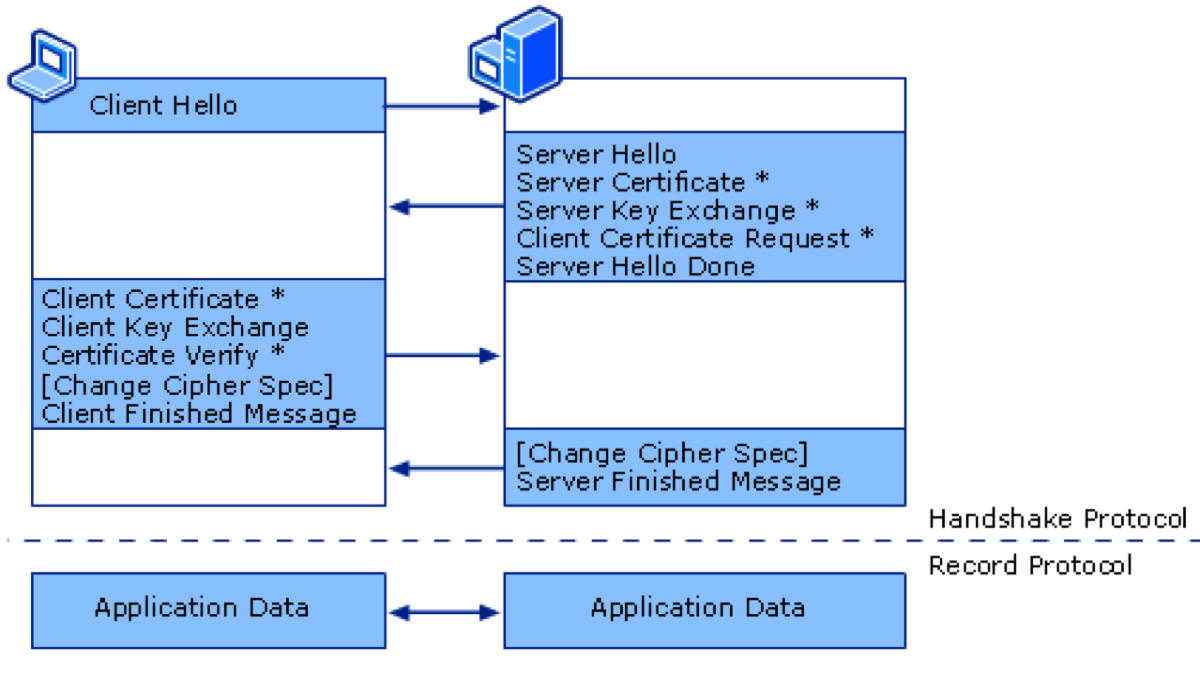
\includegraphics[width=0.7\linewidth]{images/tls_handshake}
	\caption{TLS Handshake}
\end{figure}
\begin{enumerate}
	\item Client Hello: Der Client öffnet die Verbindung und sendete folgende Dinge an den Server
	\begin{itemize}
		\item Zufällig generierte Zahl (Nonce)
		\item Liste von ihm unterstützter Verschlüsselungsverfahren für den Schlüsselaustausch
		\item List von ihm unterstützte Verschlüsselungsverfahren für die symmetrisch Verschlüsselung
		\item Liste von ihm unterstützte Hash Verfahren (HMAC) $\Rightarrow$ für Integrität
		\item Höchste unterstützte SSL/TLS Protokoll Version
		\item Session ID (falls bereits eine Verbindung in der Vergangenheit aufgebaut wurde)
	\end{itemize}
	\item Server Hello: Server antwortet und sendet folgende Dinge zurück an den Client
	\begin{itemize}
		\item Zufällig generierte Zahl (Nonce)
		\item Die Session ID 
		\item Zertifikat (enthält den Public Key)
		\item Die ausgewählten Hash- und Verschlüsselungsverfahren aus der Auswahl des Clients
	\end{itemize}
	\item Client Key Exchange: Der Client überprüft das Server Zertifikat auf seine Korrektheit und verwendet dann den Public Key aus dem Server Zertifikat um den symmetrischen Schlüssel für die weitere Kommunikation an den Server zu senden.
	\item Optional kann sich der Client gegenüber dem Server identifizieren, indem er sein X509
	Zertifikat zum Server sendet.
	\item Change Cipher Spec: Der Server teilt dem Client mit, dass er per sofort nur noch mit der ausgewählten Cipher Suite kommuniziert. Die Daten werden nun mit dem symmetrischen Key verschlüsselt. Dieser Schlüssel ist dem Server und Client bekannt. Die verschlüsselten Daten werden zusätzlich mit einem keyed-Hash MAC (Message Authentication Code) geschützt, um die Datenintegrität zu gewährleisten. Als Key wird dabei der vorhin ausgetauschte symmetrische Schlüssel verwendet. Änderungen an den verschlüsselten Daten können somit detektiert werden.
\end{enumerate}

\subsubsection{Session ID}
Wenn der Client und Server eine frühere Session wiederaufnehmen wollen, kann  der Client bei der ClientHello Nachricht die alte Session ID mitliefern. Wenn der Server sie akzeptiert, werden die alten ausgehandelten Parameter wiederverwendet und eine Authentisierung entfällt. Die SessionId muss zwingend beim Server und beim Client gespeichert werden.

\subsubsection{TLS False Start}
TLS False Start ist eine Erweiterung des Protokolls, die es erlaubt, dass die Daten bereits verschlüsselt übertragen werden, bevor der Handshake (Antwort der andere Seite) wirklich abgeschlossen ist. Nach dem ChangeCipherSpec werden die Daten direkt verschlüsselt übertragen.

\subsubsection{Null Cipher Suites}
Cipher Suites mit NULL werten sollte niemals ausgehandelt werden dürfen. Dabei wird zwar TLS verwendet, aber im Endeffekt nichts verschlüsselt oder komprimiert. ($TLS\_NULL\_WITH\_NULL\_NULL$)

\subsection{TLS/SSL Proxy}
\begin{enumerate}
	\item Der Client enthält das Zertifikat des Proxies. Dieses Zertifikat muss meist manuell hinterlegt werden, da es nur organisationsintern gültig ist.
	\item Der Client baut eine Verbindung zum Proxy auf, welcher die Verbindung entschlüsseln und durchsuchen kann. (Für Malware Erkennung, Filter, Überwachung)
	\item Der Proxy leitet die Anfrage zum Webserver weiter und verwendet dabei das Zertifikat des Ziel Webservers
\end{enumerate}

\subsection{Perfect Forward Security}
Mit diesem Verfahren werden für jede Verbindung neue Schlüssel abgeleitet (z.B DH mit zufälligen Exponenten). Kommt zum Beispiel bei RSA der private Key abhanden können alle in der Vergangenheit aufgezeichneten Verbindungen im Nachhinein entschlüsselt werden. Mit PFS kann höchstens eine einzige Session entschlüsselt werden.

\subsection{HSTS: HTTP Strict Transport Security}
Hierbei wird HTTPS erzwungen. Ist keine HTTPS Verbindung möglich, wird die Seite nicht angezeigt. HSTS ist ein Header Feld im HTTP Header (Strict Transport Security).  

\subsection{Certificate Pinning}
Der Server sendet dem Client in einem HTTP Header mit, welches explizite Zertifikat für diese Domain gültig ist. Es wird dabei eine max-age angegeben. Neue Zertifikate für diese Domain werden während dieser Zeit nicht angenommen. Der Client bestimmt dabei die absolute max-age, die vom Server nicht überschritten werden darf. Somit wird verhindert, dass ein Angreifer die max-age Time zu hoch einstellt und somit eine Seite für längere Zeit "offline" nimmt.

\subsection{SNI: Server Name Indication}
Für den Fall das auf einem Server (eine IP Adresse) mehrere Domains betrieben werden, muss der Client zuerst das korrekt Zertifikat beantragen bevor er eine HTTPS Verbindung aufbauen kann. Dazu wird SNI verwendet. Der Client sendet dem Server den gewünschten Host, wobei der Server mit dem korrekten Zertifikat des Hosts antwortet.

\subsection{OCSP: Online Certificate Status Protocol}
OCSP ist ein Netzwerkprotokoll mit welchem der Status von einem X.509 Zertifikat in Echtzeit abgefragt werden kann. Dieser Service stellen die CA's zur Verfügung.  

\subsection{CRL: Certificate Revocation List}
In der CRL wird die Ungültigkeit von Zertifikaten beschrieben. Sie ermöglicht es, festzustellen, ob ein Zertifikat gesperrt oder widerrufen wurde und warum. Die Liste umfasst die aktuellen Seriennummern der ungültigen Zertifikate. Die CRL werden von den CA's zur Verfügung gestellt und können bei dort heruntergeladen werden.

\section{IAM: Identity and Access Management}

\subsection{AAA: Authentication, Authorization, Accounting}
\begin{description}
	\item[(Identifikation)] Erfassung der Identität
	\item[Authentication] Die Authentisierung überprüft ob der User 
	derjenige ist, den er vorgibt zu sein (Username und Passwort)
	\item[Authorization] Steuert was ein Benutzer machen darf. Zugriff auf Ressourcen, gesteuert durch Rollen
	\item[Accounting] Logging / Protokollierung der Tätigkeiten auf dem System
\end{description}

\subsubsection{Authentication}
Bei Fingerabdruckscanner gibt es False Acceptance und False Rejection Rates für eine gewisse Schwelle wann ein Finger akzeptiert wird. Es ist also immer ein Abschätzen wie die Schwelle gewählt wird. Es gibt aber nicht wirklich ein Optimum.
\begin{itemize}
	\item Passwort, PIN
	\item Client Certficate, RSA Token
	\item Fingerprint (mit Pulserkennung), Iris Scan, Retina Scan (ist zuverlässiger wie Iris Scan), Voice (unzuverlässig), Gesichtserkennung, Venen Scan
\end{itemize}

\paragraph{FRR: False Rejection Rate / FAR: False Acceptance Rata}
\begin{figure}[h]
\centering
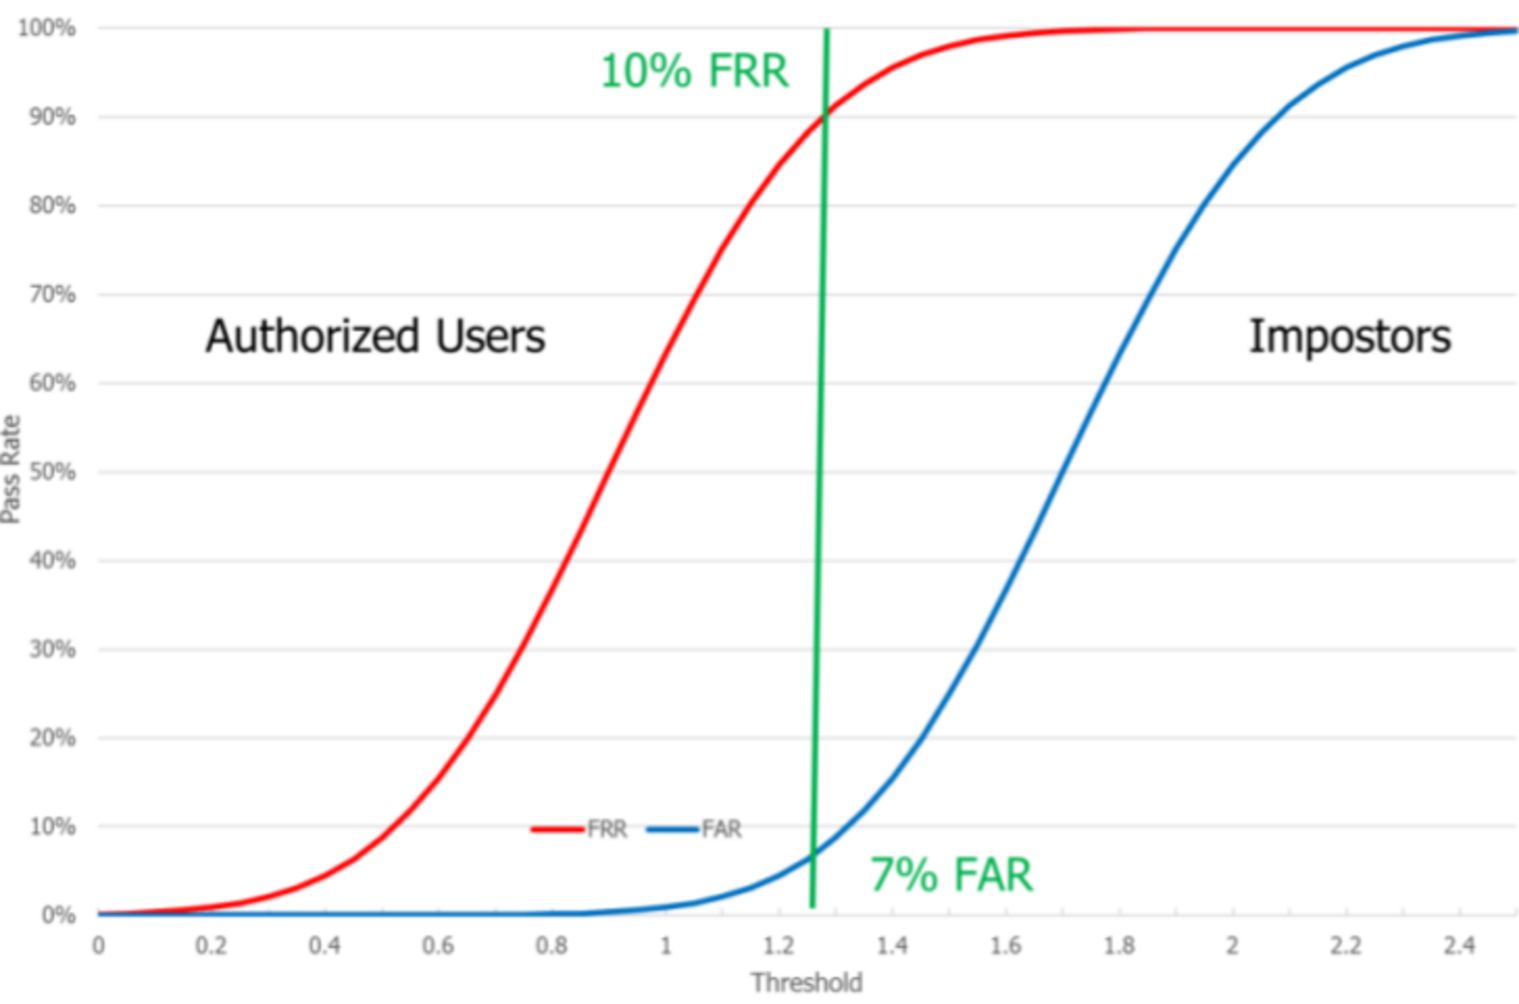
\includegraphics[width=0.5\linewidth]{images/false_rates}
\caption{False Rates}
\end{figure}

\subsection{Passwörter}
Grundlegend wird das Passwort mit einer Einwegfunktion gehashed. Der resultierende Hash wird dann zusammen mit dem Benutzernamen abgelegt. Möchte sich ein User Authentifizieren, wird erneut ein Hash über die Eingabe gemacht und mit abgelegten Hash verglichen. Um Dictionary-Attacken zu verhindern sollte zusätzlich zum Hash noch ein Salt abgelegt werden. (ACHTUNG: Salts helfen nicht gegen Offline Attacken. Da ein Salt theoretisch public ist, kann einfach eine neue Rainbow Tabelle mit dem Salt berechnet werden.)

\begin{itemize}
	\item Windows: $C:\backslash Windows\backslash system32\backslash config\backslash SAM$ (Security Account Manager)
	\item Unix: /etc/passwd (User ID's)
	\item Unix: /etc/shadow (Password Hashes)
\end{itemize}

\subsubsection{Entropie}
Je mehr unterschiedliche Symbole ein Alphabet besitzt, welches für ein Passwort verwendet wird desto besser. Aktuell gelten Passwörter mit einer Länge von 13 Zeichen druckbare Symbole (96 Symbole) als sicher. Ab 20 Zeichen spricht man von extrem sicher.

\paragraph{Berechnung:}
\begin{align}
	\begin{split}
	\text{Entropie pro Zeichen} &= log_2(\text{Anzahl Zeichen im Alphabet}) \\
	\text{Schlüsselstärke (Bit)} &=  \text{Entropie pro Zeichen} \cdot \text{Schlüssellänge}
	\end{split}
\end{align}

\subsubsection{Angriffe}
Passwörter lassen sich über verschiedene Wege herausfinden
\begin{itemize}
	\item Tools wie John the Ripper (CPU), DaveGrohl (CPU), oclHashcat (GPU) probieren Wörter aus Wörterbücher und deren Verfremdungen (Abänderungen) sowie Well Know Passwörter (Gemäss Wahrscheinlichkeit) einfach durch.
	\item Social Engineering
	\item Raten
	\item Keylogger
	\item Sniffing
\end{itemize}

\subsection{Salting}
Wenn man gehashte Passwörter speichert muss man unbedingt einen Salt verwenden um sich gegen Rainbow Table Attacks zu schützen. Ein Salt ist eine zufällige Zeichenkette die für jeden Benutzer unterschiedlich ist. Es muss davon ausgegangen werden, dass der Salt öffentlich ist, grundsätzlich sollte der Salt aber trotzdem geheim gehalten werden. Der Salt wird zusammen mit dem wirklichen Passwort dem Hash übergeben.


\subsection{Challenge Response Verfahren}
Mit einem Challenge Response Verfahren wird verhindert, dass Replay Attacken möglich sind. Beim Authentifizieren besteht das Problem, dass ein Angreifer den übermittelten Passwort Hash abgreifen und erneut an den Server senden kann. Es könnte sich damit beim Server authentifizieren. Beim Challenge Response Verfahren wird zusätzlich ein einmaliger Wert (Nonce, z.B die Zeit) in den Hash gemischt, was Replay Attacken unmöglich macht. 
\subsubsection{Ablauf}
\begin{enumerate}
	\item Server sendet eine sogenannte Challenge an den Client. Diese Challenge ist eine Nonce, das heisst ein zufälliger Wert der sich nie wiederholen darf. Es ist auch möglich ein einfachen Counter (z.B die Zeit) zu verwenden.
	\item Der Client erstellt eine eigene Nonce und übergibt diesen zusammen mit dem Benutzernamen und der Server Nonce der Hashfunktion. Die Hashfunktion berechnet mit dem Benutzerpasswort die MAC (Keyed Hash)
	\item Response: Client sendet Benutzername, Client Nonce und berechnete MAC an Server zurück.
	\item Server berechnet ebenfalls mit Benutzername, User Nonce und Server Nonce den MAC.
	\item Server vergleicht die beiden MAC (Hashes) miteinander
\end{enumerate}

Es gibt zwei Varianten dieses Verfahrens, nämlich eine synchrone und eine asynchrone:
\begin{description}
	\item[Keyed Hash / MAC] Diese Variante bedingt dass der Server das Passwort in Plaintext verfügt.
	\item[Public Key Digital Signature] Bei dieser Variante wird der Hash mit dem private Key des Clients verschlüsselt und diese resultierende Signatur an den Server übertragen. Der Server entschlüsselt die Signatur und kann dann wieder die beiden Hashes vergleichen
\end{description}
\begin{figure}[h]
\centering
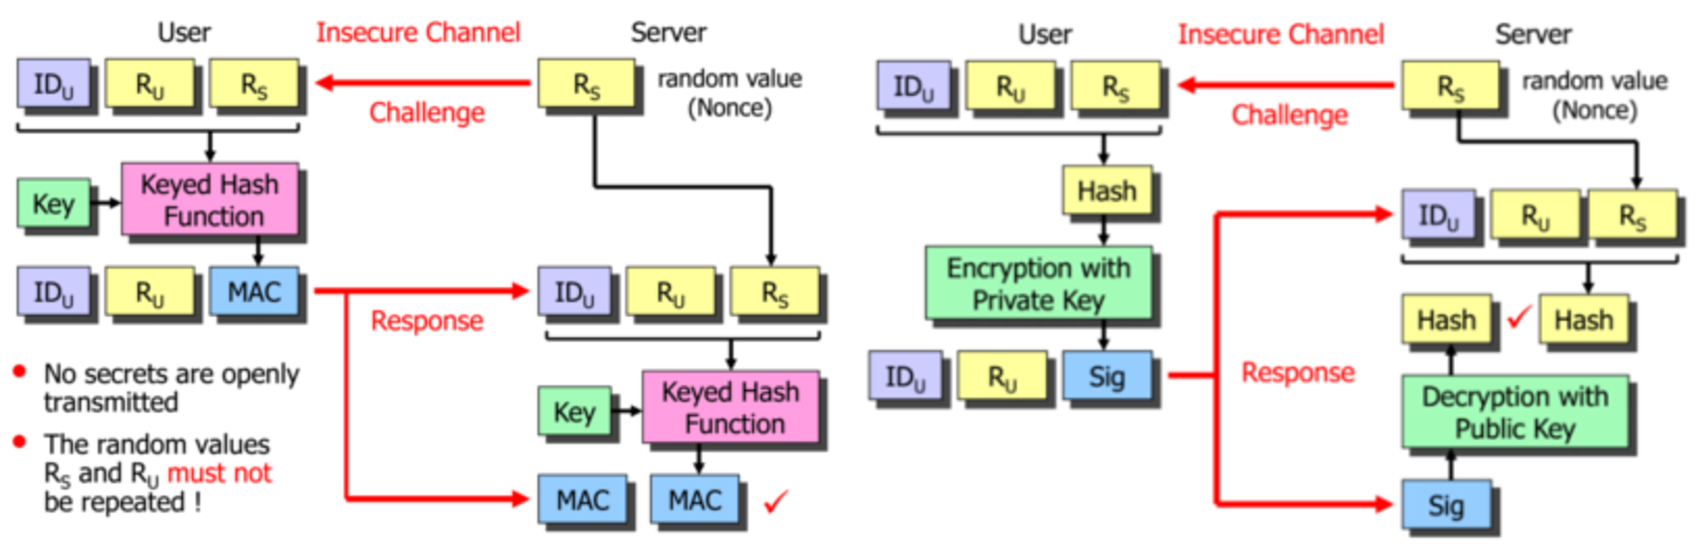
\includegraphics[width=1\linewidth]{images/challenge_response}
\caption{Challenge Response Ablauf}
\end{figure}

\subsubsection{Angriffe}
\begin{description}
	\item[Known Plaintext Angriff] \hfill \\ Übertragene Challenge sowie die zugehörige Response wird gesnifft und versucht auf das Passwort zu schliessen. 
	\item[Wörterbuchangriff] \hfill \\ Hier rät der Angreifer das Passwort, verschlüsselt damit die Zufallszahl und vergleicht sein Ergebnis mit der Response
\end{description}

\subsection{Kerberos}
Kerberos hat sich als Standardprotokoll für Single-Sign-On (SSO) in Unix- und Windows-Netzwerken etabliert. Dabei authentifiziert sich ein Benutzer einmal beim zentralen Key Distribution Center (KDC), die weitere Authentifizierung gegenüber anderen Diensten erfolgt automatisch ohne Interaktion des Clients. Kerberos nutzt das Challenge/Response Protokoll. Als Challenge wird die aktuelle Uhrzeit verwendet (Nachteil Zeitsynchronisation, Vorteil: Challenge vom Server zum Client kann eingespart werden, )

\section{Disk Encryption}
Aktuell eignet sich VeraCrypt als vertrauenswürdiges Tool für die Verschlüsselung von Festplatten. Bei der Einreise in ein Land wie z.B der USA kann es vorkommen, dass einem die Einreise verweigert wird, solange man den Schlüssel für die Entschlüsselung nicht herausrückt. Um trotzdem besonders schützenswerte Daten geheim zu halten, können sogenannte Hidden Container angelegt werden. Diese sind innerhalb eines normalen VeraCrypt Volumen eingebettet und befinden ganz am Schluss des reservierten Speicherbereichs. Da ein VeryCrypt Volumen immer mit Random Daten gefüllt ist, bemerkt man auf den ersten Blick auch nicht, dass innerhalb des Parent Container noch ein Hidden Volume existiert.

\subsection{CBC Ansatz}
Beim Cipher Block Chaining Ansatz wird jeweils der Plaintext mit dem vorhergehenden Chiffrat mit XOR verknüpft und anschliessend mit dem synchronen Schlüssel verschlüsselt. Für den ersten Block wird ein Initialisierungsvektor verwendet. Damit bei einer Änderung nur ein bestimmter Teil der Festplatte entschlüsselt werden muss, wird immer ein ganzer Festplattensektor verschlüsselt. Ein Sektor ist normalerweise 512 Bytes gross. Bei einer AES Blockgrösse von <16Byte ergeben sich so 32 Blöcke pro Sektor. Der CBC Ansatz wird heutzutage nur noch von Bitlocker von Microsoft verwendet. Bitlocker ist nicht quelloffen und deshalb fragwürdig ob nicht irgendwelche Backdoors eingebaut sind.

\subsubsection{Angriffe}
\begin{description}
	\item[Watermarking] \hfill \\
	Beim Watermarking geht es darum, zu beweisen, dass eine bestimmte Datei auf einer verschlüsselten Festplatte zu finden ist: Das Problem beim CBC (ohne ESSIV: Encrypted salt-sector initialization vector) ist, dass der IV nach einem bekannten Muster generiert wird. (z.B wird die Festplatten Sektornummer verwendet). Das Opfer lädt sich dabei eine speziell präparierte Datei auf seine verschlüsselte Festplatte. Mit Watermarking kann nun ohne Kenntnis des Schlüssels nachgewiesen werden, dass das Muster auf der Festplatte vorhanden ist. z.B könnte man speziell manipulierte Pornographie jemandem unterschieben, um zu beweisen, dass die Person Kinderpornographie konsumiert.
	\item[Malleable Plaintext] \hfill \\
	Unter Malleability versteht man, dass ein Angreifer ein Chiffrat so umformen kann, dass die Fälschung beim Entschlüsseln eine sinnvollen Klartext ergibt. (malleable = verformbar) 
	\item[Movable Cipher Blocks] \hfill \\
	Man nimmt den Ciphertext und verschiebt diesen mit einem Low Level Tool auf einen unbenutzten Sektor der vom Betriebsystem nicht geblockt ist. Auf dem neuen Sektor werden dann alle Blöcke ausser dem ersten Block (IV fehlt) vom OS entschlüsselt.
\end{description}

\subsection{XTS-AES-Based Hard Disk Encryption}
\begin{description}
	\item[XEX:] XOR,  Encrypt, XOR
	\item[XTS:] XEX-based Tweaked-codebook mode with ciphertext Stealing
	\item[CTS: Ciphertext Stealing] \hfill \\
	CTS erlaubt dass der Klartext mit einem Blockcipher ohne Padding verschlüsselt werden kann. Der Klartext ist dabei immer genau gleich lang wie das Chiffrat. Bei dem Verfahren sind nur die letzten beiden Blöcke betroffen:
	\begin{enumerate}
		\item Zuerst werden alle Blöcke bis zum Letzten wie gewohnt verschlüsselt
		\item Anstatt den letzten Block zu padden, wird vom vorletzten Block so viel Chiffrat geklaut/entfernt, dass der letzte Block die benötigte Blocklänge von 16Byte erreicht.
		\item Der letzte Block kann nun auch verschlüsselt werden
		\item Beim Entschlüsseln muss dann gezwungenermassen der letzte Block zuerst entschlüsselt werden, damit der entfernte Cipher wieder dem zweitletzten Block zurückgegeben werden kann. 
		\item Alle fehlenden Blöcke können dann wieder wie gewohnt entschlüsselt werden.
	\end{enumerate}
	 Ciphertext Stealing findet hauptsächlich Anwendung in der Dateiverschlüsselung. Bei der Festplattenverschlüsselung ist Ciphertext Stealing nicht nötig, da Festplattenblöcke von 512Bytes immer vielfache der AES Blockgrösse von 16Byte sind ($16 \cdot 32 = 512$)
\end{description}
Der deutlich sicherere XTS Ansatz wird heutzutage von den meisten grossen Verschlüsselungssoftware verwendet. Er ist im Gegensatz zum CBC Ansatz resistent gegenüber Watermarking und Cipherblock Move Attacken. XTS verwendet zwei AES-Schlüssel. Ein Schlüssel wird zur AES-Blockchiffrierung verwendet und der andere verschlüsselt nach dem sogenannten Tweak-Wert. Dieser verschlüsselte Tweak wird wiederum durch die Funktionen Galois-Polynom (GF) und XOR mit dem Klartext und dem chiffrierten Text jedes Textblocks verknüpft. Die GF-Funktion sorgt für eine weitere Diffusion und stellt sicher, dass Blöcke mit identischen Daten keinen identischen chiffrierten Text enthalten. Dadurch wird erreicht, dass jeder Block seinen eigenen chiffrierten Text für identischen Klartext ohne den Einsatz von Initialisierungsvektoren und Chaining erstellt. Im Endeffekt ist der Text über zwei voneinander unabhängige Schlüssel nahezu doppelt verschlüsselt. Die Entschlüsselung der Daten erfolgt in umgekehrter Reihenfolge des Prozesses. Jeder Block ist eigenständig und nicht mit anderen Blöcken verkettet. Dies bedeutet, dass bei einer Beschädigung von gespeicherten, chiffrierten Daten nur die Daten dieses bestimmten Blocks nicht mehr wiederherstellbar sind. In Chaining-Modi können sich diese Fehler auf andere, verschlüsselte Blöcke ausweiten.
\begin{figure}[h!]
\centering
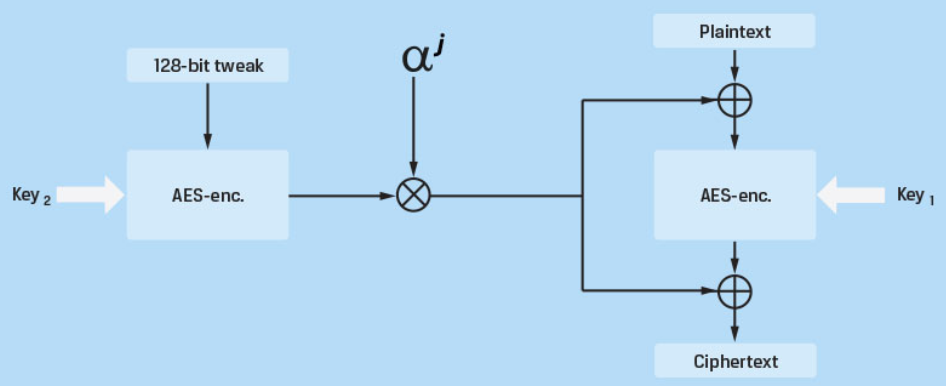
\includegraphics[width=0.6\linewidth]{images/xts_aes}
\caption{XTS-AES}
\end{figure}

\section{Email}
\subsection{S/MIME: Secure / Multipurpose Internet Mail Extensions}
S/MIME ist ein Standard für die Verschlüsselung und Signierung von E-Mails welcher von den meisten aktuellen Mailclients unterstützt wird.

\subsection{MIME: Multipurpose Internet Mail Extensions}
Es existieren zwei Content-Types für MIME. Mit dem $multipart/signed$-Format lässt sich eine Mail signieren und mit dem $application/pkcs7-mime$ lässt sie sich zusätzlich verschlüsseln. Es spielt keine Rolle ob zuerst signiert oder verschlüsselt wird. Wenn aber zuerst verschlüsselt und dann signiert wird, kann der Absender zuerst identifiziert werden, bevor entschlüsselt wird. Ansonsten bleibt dieser anonym.
  
\subsubsection{Signieren: multipart/signed}
Eine signierte E-Mail hat den Content-Type "multipart/signed". Eine Nachricht besteht immer
aus 2 Blöcken (Boundary), nämlich aus dem Inhalt der signiert werden soll und aus 
der digitalen Signatur, welche die Echtheit des Absenders bestätigt. Der Vorteil davon ist, dass wenn ein Mailclient kein S/MIME unterstützt, kann dieser den ersten Block (die Meldung) immer noch lesen. Verändert der Mailclient z.B durch unterschiedliches Encoding die Mail wird die Signatur ungültig.

\subsubsection{Verschlüsseln: application/pkcs7-mime}
Der Content-Type application/pkcs7-mime verfügt über den optionale Parameter smime-type, der die Art der Daten beschreibt:
\begin{enumerate}
	\item enveloped-data (Verschlüsselung)
	\item signed-data (Signatur)
	\begin{itemize}
		\item Die Nachricht wird im Klartext innerhalb des binären PKCS\#7 Objekts transportiert. Dies schützt die Nachricht besser von Veränderungen durch den Mailserver als der multipart/signed Content Type. Falls der Client aber kein S/MIME unterstützt kann das Mail nicht gelesen werden.
	\end{itemize}
	\item certs-only (Zertifikat)
\end{enumerate}
Ausserdem zeigt der Dateiname des optionalen, aber erbetenen Headereintrags Content-Disposition die Art der Daten an:
\begin{enumerate}
	\item smime.p7m (signierte oder verschlüsselte Daten)
	\item smime.p7c (Zertifikat)
	\item smime.p7s (Signatur)
\end{enumerate}
Ein Abschnitt mit verschlüsselten Daten enthält ebenfalls genau zwei Blöcke. Der erste enthält die benötigte Informationen zur Entschlüsselung. Im zweiten Block sind die verschlüsselten Daten enthalten. Der Mailrumpf ist komplett verschlüsselt. Wie bei PGP sind die Mailheader (auch der Betreff) dagegen unverschlüsselt und sollten daher keine vertraulichen Informationen enthalten. Zur Verschlüsselung einer E-Mail muss der Absender den öffentlichen Schlüssel des Empfängers kennen, den er beispielsweise dem Zertifikat einer zuvor vom Empfänger erhaltenen signierten E-Mail entnehmen kann. Zusätzlich empfiehlt es sich, dass sich der Absender selber auf die Verteilerliste nimmt, damit die Mail auch mit seinem Public Key verschlüsselt wird und er so seine eigene Mail später wieder lesen kann. Ebenfalls sollte immer ein Backup des Private Keys existieren, damit die Mails bei Verlust des Keys immer noch dechiffriert werden können.


% Anhänge / Infos einfügen
\appendix

% Code Listings
\lstlistoflistings

% List of figures
\listoffigures

% List of tables
\listoftables

% Bibliography
\bibliographystyle{plain} 
\bibliography{literatur}

\end{document}